
\newcommand\dive{\textmd{div}}
\newcommand\der{\textmd{d}}



\chapter{Introduction}
%some background on all astronomy/astrophysics

Humans have been captivated by the stars since the dawn of civilisation, and this fascination has driven our curiosity and drive to understand the universe around us. 
The history of astronomy is rich and diverse. 
Indigenous cultures still use the stars for navigation, seasonal calendars, and mythological stories. 
Since the invention of the modern telescope, some would say the birth of modern astronomy in the 16th century, to the launch of the James Webb \update{Space Telescope}, technology has advanced during the period that this PhD was undertaken. 
Our ability to observe and study the stars has grown in scale and sophistication. 

Each observation that we make improves our understanding of the underlying physics of the universe. 
In recent years the sheer amount of data available to astronomers has increased dramatically due in part to technological advances, such as space-based observatories, which allow us to perform large sky surveys in unprecedented detail. 
It is clear from these studies that our models of the universe are lacking in a number of important physical processes. 
One of these physical processes that are particularly not well understood is the evolution of stellar rotation\footnote{Infact a majority of models of stellar evolution completely ignore angular momentum transport}.

This introductory chapter is intended to provide context for the reader to understand the following science chapters. 
The introductory chapter is broken down into the following sections of increasing level of detail:

Section \ref{sec:history} provides a historical overview of the history of astronomical observation and briefly introduces the techniques used to observe the rotation of stars.
Section \ref{sec:evolution} reviews our current understanding of the evolution of rotation from birth, through post-main sequence evolution, to the remnants of rotating stars. Within this Section we\footnote{\update{for stylistic reason I use the word ``we" to describe work that I have led in collaboration with others.}} also describe what we call the \update{``problems of stellar rotation"} that we have attempted to address in this work.
Section \ref{sec:effects} we briefly describe the effects of the rotation of the evolution of low-mass stars.
Section \ref{sec:techniques} outlines the techniques that are employed to observe the rotation of stars.

The scientific works in this thesis are motivated by the problems in stellar rotation that are described in detail in this introduction. As a result, this introduction will overlap with the introductions of the scientific works' topics and serve as a companion for readers unfamiliar with the topic.

\section{An introduction to the observation of stellar rotation}
\label{sec:history}

\subsection{Classical observations of rotation}


In this section, we look back at the history of observing stellar rotation, how observations of stellar rotation are performed, the qualitative effects of rotation on \update{stellar evolution} and some of the problems that the big-data boom of astronomy has identified.
This discussion will provide the necessary background to our attempts to understand and constrain the astrophysical process that underlies these problems.

The history of observing the rotating stars began with observations of the Sun\footnote{as most astronomy does}. 
In approximately 1610, Galileo reported evidence of sunspots and tracked their motion in his book \update{``L'Istoria e dimostrazioni intorno alle macchie solari e loro accidenti".} 
He interpreted the motion of stellar spots on the surface of the Sun as a result of its rotation. 
Adding onto this work in 1630, Christoph Scheiner found that the stellar spots had different rotational periods at the poles and the equator, measurements that agree with modern observations of the Sun. 
\update{This was the first observation of latitude-dependent rotation, more commonly known as latitudinal differential rotation.}

The history of observing stellar\footnote{Here we make the distinction between the Sun and other stars through the use of the terms \update{``solar" and ``stellar"} respectively} rotation can be traced back to the early 20th century when astronomers first discovered that some stars they observed were rotating. 
They came to this conclusion through spectroscopic observations \citep{elvey_contours_1929, struve_stellar_1930, struve_axial_1930}.
\update{They found that lines in their spectra were broadened due to the Doppler effect, a technique used to this day.}

Around this time, astrophysicists such as Eddington \citep{eddington_conditions_1918,eddington_internal_1926,eddington_internal_1929}, Milne \citep{milne_equilibrium_1923}, von Zeipel \citep{von_zeipel_radiative_1924}, and others delved into the theoretical aspects of the impact of rotation on stars.
To simplify their work, they identified the effects of rotation on stellar structure, energy generation, shape and luminosity. 
Further, \update{they argued that} rotation induces mixing in stars that can transport \update{material in stars, leading to enhanced chemical mixing and angular momentum transport}.
Advances in computational capabilities allowed astronomers to study the impact of rotation on the mixing of elements within stars in greater detail. 
Enhanced mixing leads to an increased lifetime on the main sequence, hydrogen-rich material is transported to the core, and can create isotope anomalies, such as changes in the isotopic ratio $^{12}$C/$^{13}$C, nitrogen, oxygen and lithium enhancements \citep{maeder_evolution_2000,heger_presupernova_2000,charbonnel_lithium_1994}.
Their results underlay our modern understanding of the impacts of stellar rotation on stellar evolution.

\update{In the following decades, technological advances allowed for more precise photometric observations of stars.}
This paved the way for two techniques to obtain measures of the rotation of stars: measurements of the quasi-periodic flux modulations due to stellar activity and asteroseismology.

\update{Like the Sun, stars were to exhibit magnetically active regions\footnote{Magnetically active regions can have varying effects on the flux of stars. Those regions can be brighter (faculae), darker (spots) and induce emission in Ca II H \& K and H $\alpha$ lines}. 
These regions cannot be \update{directly imaged} on the surface of stars other than the Sun. 
However, rotational modulation of magnetically active regions on the surfaces of active stars produce quasi-periodic variations in the disk-integrated flux, generally through magnitude variations due to induced brightness variations.
Measuring the period of brightness variation is used as a proxy for the rotation period\footnote{It is important to note here that the rotation period - time taken for one rotation -  and rotation rate - frequency of rotation - of a star are not the same quantity. They are inversely related} of a star.
Unlike the spectroscopic technique - where the inclination angle modulates the rotation rate  - the rotational periods from stellar spot brightness modulations are more accurate to the star's actual rotation rate.}

\update{Ground-based time-domain photometric surveys have yielded numerous rotation period measurements for stars in young clusters.
However, the limited precision of the telescopes and low cadence of time-sampling achievable from the ground are insufficient to detect rotational modulation in older, less active stars.
For many years, the Mount Wilson program monitored the emission in the cores of the Ca II H\& K lines for a large number of low-mass stars over a 20-year period \citep{wilson_probable_1963}.
The cadence of observations by this mission was on the order of days and resultingly became the main source of rotation period measurements for field stars.
This changed with the advent of space-based photometric missions such as \corot \citep{baglin_corot_2003}, \kepler \citep{borucki_kepler_2010, howell_k2_2014} and \tess\ \citep{ricker_transiting_2014}.
These missions have collectively gathered sub-mMag precision photometry with short cadence observations (time scales between observations on the scale of minutes) over baselines from months to years, which have resulted in the largest high-precision catalogues of rotational periods of low-mass main-sequence stars available \citep{mcquillan_rotation_2014}.}

Determining the rotation period of a star from stellar spots requires intermittent photometric measurements of stars - known as long-cadence observations - over the time scale of months. 
On the other hand, measurements made on the order of minutes - known as short cadence observations - reveal the internal structure of stars.
Like bells, stars \update{``ring"} - or, more accurately, pulsate, and thus vary in brightness -  at particular frequencies related to the structure of the star.
By measuring those frequencies, we can infer the internal structure of a star: for example, the density-sound speed profile of the star.
Rotation introduces what are known as rotational splittings to the frequency profile.
Rotational splittings vary between asteroseismic modes but are a weighted average of the rotation rate dependent on the structure of the star. 
Unlike brightness modulations from stellar spots and spectroscopic inference of surface rotation rate, asteroseismology can probe the rotation profile inside a star.

Modern observations with asteroseismology\footnote{and helioseismology for the Sun} have also found that the Sun, and most post-main sequence stars, exhibit differential rotation along the radial axis - known as radial differential rotation.
Measurement of the rotation profile of post-main sequence stars has allowed us to probe these stars' internal mixing and angular momentum transport. 
It is important to note, however, due to the large amount of photometric data required to perform in-depth asteroseismic inference, \update{the number of stars with internal rotation profile measurements} is only on the order of 100\footnote{at the time of writing} \citep{li_asteroseismology_2020,li_asteroseismology_2020-1}, and the constraints that state-of-the-art data can provide are limited.

As a result, these techniques have made several fundamental discoveries about the evolution of stellar rotation.
For example, it was found that the rate at which a star's surface rotates slows with time \citep{skumanich_time_1972}.
As a result, measuring the stellar rotation can provide a measure of the age of a star\footnote{This is a contentious claim, our understanding of the evolution angular momentum transport of stars is consistently growing}.
A number of other features of stellar rotational evolution have been identified that we will outline in this Chapter - as well as a number of problems that require investigation that we will attempt to resolve in this Thesis.

\subsection{Modern observations of rotation}

Here we will briefly reflect on current methods of observing rotation in stars, where these methods are most conducive to understanding the evolution of rotation and their limitations.
The three standard techniques of observing rotation in stars: measurement of the surface rotation period from stellar brightness oscillations owing to stellar spots, spectroscopic derivation of inclination projected surface velocity from doppler broadenings, and asteroseismology of rotational splittings.
We will refer to these techniques by their data products: stellar spot rotation periods, spectroscopic rotation velocities, and asteroseismic rotation rates, respectively, for brevity.
% We discuss these techniques more thoroughly in Section \ref{sec:techniques}.
The results we discuss in this Section come from the inference of rotational evolution from stellar spot rotation.
This results from two factors: stellar spot rotation periods are more accurate and less data and computationally intensive than their spectroscopic and asteroseismic counterparts.

While spectroscopic rotation velocities have been inferred for orders of magnitude stars, the observed rotation rate is modulated by the inclination angle of the star relative to the observer ($v\sin{i}$).
Constraining the evolution of rotation through spectroscopic rotation velocities of stars is only fruitful with independent constraints to stellar inclination.
The stellar inclination is often difficult to measure as it requires either that the star is in a binary\footnote{and that the rotation axis aligns itself with the binary orbital inclination, which may always be the case \citet{albrecht_banana_2011,albrecht_banana_2013}} or that the star is intensively asteroseismically studied.
As a result, only a few studies of the evolution of rotation rely on this data.

On the other hand, determining the rotation rate of stars with asteroseismology is computationally and data-intensive.
We will discuss the difference in computational intensity in more detail when we outline how these methods are performed.
Here we will focus on the difference \update{in required amount of data}.
Obtaining high signal-to-noise asteroseismic signals of rotation requires short-cadence observations of stars over an observation period \update{on the order of years} \citep{deheuvels_seismic_2014}.
%@andy It;s a bit of both, we are at a point with tess data where we are starting to see high S/N asteroseismic signals. It seems thats the threshold which just happens to line up with the kepler mission length
Short-cadence data is required because the oscillation frequencies of stars must be \update{shorter} than the Nyquist frequency of the observations.
In the \kepler{} field, the cross-section of stars with both short-cadence observations and those observation periods long enough to obtain a high enough \update{signal to noise} to perform asteroseismic inference \update{does not include a large number of stars}.
Further, only limited constraints can be placed on the surface rotation rate from asteroseismology during the main sequence.
 stars only express \update{pressure}-mode\footnote{See Section \ref{sec:techniques}} solar-like oscillations with long lifetimes, which can only probe the structure of the convective surface region.
Long mode lifetimes result in \update{broadened oscillation peaks in the power spectrum}.
\update{Stars also spend the majority of their lifetime slowly rotating.}
This results in rotational broadenings of the oscillations rather than distinct rotational splittings.
Without precise measurements of the rotational splittings for many oscillation modes, precise inference of the surface rotation rates of stars is limited.

The inefficiency of asteroseismic inference of rotation rates along the main sequence is best exhibited in \citet{hall_weakened_2021}, who observed the asteroseismic surface rotation rates of 91  stars.
Figure 2. in \citet{hall_weakened_2021} compares the stellar spot rotation period with the surface rotation period from asteroseismic inference of the rotation profile.
The surface rotation periods generally agree, confirming that the surface brightness oscillation period from stellar spots is indeed the surface rotation period.
However, the rotation periods obtained from asteroseismology are much less precise than their stellar spot rotation period counterparts.
Despite requiring much more data, the information provided by this technique is limited compared to stellar spot brightness modulation periods.

Stellar spot rotation period measurements can be made from long-cadence data with observation periods as low as 90 days \citep{mcquillan_rotation_2014}.
The technique employed to determine the rotation period is much less computationally intensive than required for asteroseismic inference of rotation rates.
Through the combination of various photometric missions, \kepler{} \citep{mcquillan_rotation_2014, santos_surface_2021}, \ktoo{} \citep{santos_surface_2021}, Zwicky Transient Facility (\ZTF) \citep{lu_bridging_2022}, and \gaia{} Data Release 3 (DR3) \citep{distefano_gaia_2022}. %todo reference% ~500,000 stars have had their stellar spot rotation periods measured.
We show the rotational period distribution against colour (\gaia{} DR3 $B_P - R_P$) of the representative \kepler{}, \ZTF{} and \gaia{} DR3 rotational period samples in the top left, top right, bottom left and bottom right panels of Figure \ref{fig:rot_comp} respectively.

\begin{figure}[h]
    \includegraphics[width=\textwidth]{Figures/intro_figures/rot_comp.png}
    \caption[2D normalised histograms of representative \kepler, \gaia, and \ZTF{} rotational period distributions]{Normalised 2D histograms of the \kepler{} \citep{mcquillan_rotation_2014} (top), \gaia{} DR3 \citep{distefano_gaia_2022} (middle), and Zwicky Transient Facility (\ZTF) \citep{lu_bridging_2022} (bottom) samples. Each sample probes a different area of the rotational period against colour space with some overlap. This expands our knowledge of the evolution of rotation to different types of stars. \update{Their agreement in overlapping regions of the rotational period distribution also confirms their independent accuracy.}}
    \label{fig:rot_comp}
\end{figure}

The stellar spot rotation periods that are obtained from each of these missions are suited to observe particular masses and rotation period regimes along the main sequence.
This results from the underlying telescope parameters, the scanning technique employed, and each mission's observation cadences \citep{distefano_determination_2012}.
%The Gaia DR3 rotation period sample exhibits spurious periods centred around 0.5, 18, 25, 32 and 49d.
%\citet{distefano_gaia_2022} suggest that the non-uniformity of the Gaia sampling could be the cause of these peaks.
%@andy: I was wrong about this, this is before processing.
Comparing the rotational period distributions in Figure \ref{fig:rot_comp} we observe a few notable features and limitations from each mission.
\update{For example, before post-processing the Gaia DR3 rotation period sample exhibits spurious periods centred around 0.5, 18, 25, 32 and 49d (compare Figures 17, 18 and 19. in \citet{distefano_gaia_2022}) due to the non-uniformity of \gaia{} sampling.
Period detections at these periods or at fundamental over and undertones should be treated with caution.
Another example comes in the form of the \kepler{} instrument's pixel-level temperature changes can produce periodic variability with a period of approximately 10 days, falling within the range of rotation periods of young low-mass main-sequence stellar rotators. Rotation period observations close to this period should therefore also be treated with caution.}

Different missions can also have different selection functions depending on their intended science goals.
\kepler{} mainly targeted solar-like\update{, relatively higher mass ({$M\sim M_\odot$),}stars.}
As a result, in the \kepler{} sample, there is a lack of measured periods for M dwarfs and fast-rotating young stars.
On the other hand, the \ZTF{} and \gaia{} samples did not have this targeting bias and have a non-specific untargeted approach.
The \ZTF{} and \gaia{} samples probe the rotation periods of the comparatively lower-mass (redder) stars.

\update{Due to the \kepler{} mission's long baseline, but usually long-cadence data, it is biased towards the observation of long periods (P $<$ 10 d).
The Gaia DR3 rotation sample is, as a result of the Gaia scanning law, mostly suited to detect periods of rapidly rotating stars (P $<$ 5 d).
While, due to the long observation baseline, the \ZTF{} mission was more suited to observe longer rotation periods.
Combining the results of these missions, we can accurately probe the evolution of rotation along the main sequence for a wider range of stellar parameters than the individual missions permit.}

Most of what we know about main-sequence stellar rotational evolution arises from measuring stellar spot rotation periods.
However, the technique is limited by the requirement for stars to express stellar spots to be effective - a limitation that is invoked several times to explain phenomena discussed later in this Section. 
\citet{mcquillan_rotation_2014} attempted to measure the stellar spot rotation periods of solar-like stars in the \kepler{} sample.
In this work, they recovered the rotation period of ~20\% of stars with long cadence observations: 34,000 detected rotation periods out of 133,000 selected stars in the sample.
On the other hand, \citet{distefano_gaia_2022} places the efficiency of the Gaia DR3 period detection pipeline at $\sim$0.4\%.
They argue that the detection efficiency is non-constant and, in fact, a function of stellar magnitude, the amplitude of the rotational modulation, the stellar rotation period and the ecliptic latitude.
There may be regions of evolution where the stellar spot rotation period does not effectively probe rotational evolution.


\section{Evolution of Rotation}
\label{sec:evolution}

\update{Here we describe the evolution of rotation in low-mass stars from birth until the end of the post-main sequence.}

\subsection{From birth to the terminal age main sequence}

All matter in the universe has some angular momentum. 
Stars are born in the core of spinning molecular clouds from the infall of matter due to gravity. 
As a result, all stars are rotating.
The amount of angular momentum a star is born with may depend on the cloud from which it was formed.

At the beginning of the pre-main-sequence (PMS) phase, a young star is typically surrounded by a disk of gas and dust from which it is accreting material.
The accretion process can lead to an increase in the rotation rate of the star, as the angular momentum of the infalling material is transferred to the star.
However, as the star grows in size and mass, its magnetic field becomes stronger, which can slow down its rotation through the process of magnetic braking.

One key feature of PMS rotational evolution is the \update{``}disk-locking" phenomenon, in which the star's rotation becomes locked to the rotation of the disk \citep{eggenberger_angular_2012}.
This occurs when the star's magnetic field is strong enough to interact with the disk, causing the star and disk to rotate together.
Disk-locking can help to explain why some PMS stars have relatively long rotation periods, even though they are young and should be rotating rapidly due to the effects of accretion.

The interplay between accretion and magnetic braking can result in a complex evolution of the rotation rate of a young star during the PMS phase \citep{gallet_improved_2013}.
Observations of young stars in star-forming regions have revealed that the rotation rates of PMS stars span a wide range, with some stars spinning rapidly and others rotating slowly.
We show this complex relationship in Figure \ref{fig:pms_ms_evo}.
Compared to the main sequence where stars generally spin-down due to surface winds, the median rotation rate of PMS cluster is relatively constant with age.

\begin{figure}
    \includegraphics[width=\textwidth]{Figures/intro_figures/pms_evo.png}
    \caption[Angular rotation rate distributions of low-mass young open clusters and the Sun over time.]{Angular rotation rate (relative to solar) distributions of low-mass young open clusters and the Sun. Inverted triangles, triangles, and squares represent the 25$^{th}$, $50^{th}$, and 90$^{th}$ percentiles. Open circle denotes the present value of the rotation rate of the Sun. Median (50$^{th}$ percentile) values indicate that the rotation rate of cluster is approximately constant with age, despite the spin-up by accretion. In order of increasing age (left to right) the clusters are ONC (1 Myr) \citep{herbst_stellar_2002}, NGC 6530 \citep{henderson_time-series_2012}, NGC 2264 (2 Myr) \citep{affer_rotation_2013}, NGC 2362 (5 Myr) \citep{irwin_monitor_2008}, h PER (13 Myr) \citep{moraux_monitor_2013}, NGC 2547 (40 Myr) \citep{irwin_monitor_2008}, Pleiades (120 Myr) \citep{hartman_large_2010}, M50 (130 Myr) \citep{irwin_monitor_2009}, M35 (150 Myr) \citep{meibom_slar_2009}, M37 (550 Myr) \citep{hartman_deep_2009}, Praesepe (578 Myr) \citep{delorme_stellar_2011}, Hyades (625 Myr) \citep{delorme_stellar_2011}, and NGC 6811 (1 Gyr) \citep{meibom_kepler_2011}.  Sourced from \citet{gallet_improved_2013},  Figure 1.}
    \label{fig:pms_ms_evo}
\end{figure}

While many main-sequence stars have had their rotation rates measured, their ages are not well-constrained.
Resultingly the evolution of rotation with age is also not well-constrained.
Observations of young open clusters' main-sequence stellar surface rotation from the \kepler{} mission suggest that angular momentum transport over a star's lifetime is consistent between clusters.
The distribution of rotational periods of stars has considerable overlap between clusters \citep{spina_how_2020, curtis_when_2020}. 
Figure \ref{fig:cluster_rotational_periods} shows the distribution of rotation rates of some open clusters.
In this Figure, we can observe some significant aspects of the evolution of angular momentum in stars.

\begin{figure}[h]
    \includegraphics[width=\textwidth]{Figures/intro_figures/cluster_kepler.png}
    \caption[Cluster rotational periods against effective temperature]{Scatter plot of various cluster rotational periods against effective temperature overlayed on the \kepler{} \citep{mcquillan_rotation_2014} rotational period sample.
    The agreement between low mass Praesepe and NGC6811 periods implies mass-dependent core-envelope coupling for young ($<$1 Gyr) stars.
    Sourced from Top left panel of Figure 7 in \citet{curtis_when_2020}.}
    \label{fig:cluster_rotational_periods}
\end{figure}

The surface rotational period increases over time for stars $<$1.1 $M_{\odot}$.
Within this range of masses, angular momentum is lost from the convective surface through mass loss and interactions of the star's magnetic field and the lost ionised material through stellar winds, known as magnetic braking.
Through observations of the Pleiades, Ursa Major, and Hyades stars and the Sun, \citet{skumanich_time_1972} derived the proportional relation between the rotational rate of stars and the inverse square of their age: $\omega(t) \propto t^{-1/2}$.
This proportionality forms the standard for expected rotational evolution and for what is known as gyrochronology - measuring the ages of stars from their rotational rate.

Outside the $\sim$0.4 and 1.1 M$_{\odot}$ range, the rotation period also decreases, albeit slower, with much more complex relationships with time.
Above $\sim$ 1.1 M$_{\odot}$, known as the Kraft break \citep{kraft_studies_1967}, stars have shallower convective envelopes and are believed to have less efficient magnetic dynamos which induce strong magnetic fields.
Resultingly, the magnetic braking in these stars is less efficient, and these stars continue to rotate rapidly throughout most of their main-sequence lifetimes. 
\update{Below 0.4 M$_{\odot}$ stars are fully convective and angular momentum is efficiently transported throughout the star.}
A greater amount of angular momentum needs to be removed to slow the star's rotational rate, compared to stars that are not fully convective.
The main sequence rotational evolution of stars with mass $>$1.3 M$_{\odot}$ is unprobed.
Above this mass, stars have no convective envelope, and thus, they do not express stellar spots nor solar-like oscillations that can be used to probe the surface rotation rate.
Theoretical modelling of the rotational evolution of high-mass stars is a substantial area of research in which observations of stellar parameters such as chemical abundances must independently constrain angular momentum transport rather than observations of stellar rotation.
As this work has a stronger focus on observing the rotation of stars, these results will not be discussed here.
For more information, we suggest reviews of astrophysical models of high-mass stellar rotational evolution, e.g. \citet{heger_presupernova_1998,maeder_evolution_2000,maeder_physics_2009}.

Until recently, it was assumed that there was little to no angular momentum transport between the radiative core and convective surface of main-sequence stars in the between $0.4 \ < \ M_{\odot} \  < \ 1.1$ range. 
Helioseismic observations of the Sun suggest that only the stellar surface undergoes rotational braking, and the core remains rotating rapidly.
\update{This suggests that minimal angular momentum transport occurs between the core and the surface during the main sequence.}
However, open cluster rotation period observations suggest that Skaumanich-like rotational evolution alone does not explain the observed distributions of rotation periods with mass \citep{spada_competing_2020}.

\citet{spada_competing_2020} proposed that mass-dependent angular momentum transport between the core and the surface was required to explain observations of young ($<$ 1 Gyr) open cluster rotation period distributions.
In their work, they argue that clusters contain two sequences of stars: a sequence of relatively slower rotators, following the expected coherent slowing of rotation rate \update{expected by} the Skaumanich relation, and a sequence of lower mass stars that appear to have a constant rotation rate between clusters of different ages.
They compared the observations of the $\sim$700 Myr old Praesepe and the 1 Gyr old NGC 6811 clusters.
Figure 1 in \citet{spada_competing_2020} compares the rotation period distribution of the Pleiades (120 Myr), Praesepe (670 Myr), and NGC 6811 (1 Gyr).
Comparing observed rotation periods, they find that higher mass stars (${>\,1 \ M_{\odot}}$) that are on the slow rotator sequence of the older NGC 6811 have longer periods than their counterparts in the younger Praesepe, as Skaumanich rotational evolution suggests.
On the other hand, the two clusters' rotational periods are indistinguishable at lower masses ($<$ 0.8 $M_{\odot}$).
In other words, low-mass stars have not been spinning down at all in the intervening 300 Myr. 
They argue that behaviour manifests mass-dependent core-envelope coupling - angular momentum transport between the core and the surface - briefly compensating for the loss of angular momentum due to wind braking at the surface.
They develop a semi-analytical model of the rotational period's evolution with a star's age and mass tuned with the observations of stellar cluster rotational period distributions.
This notably improves the accuracy of gyrochronology compared to the Skaumanich relation, especially for younger low-mass stars.

The slow spin down rates of fast rotating stars could \update{instead} be related to saturation of the angular momentum loss due to stellar winds \citep{johnstone_stellar_2015, johnstone_stellar_2015-1,gallet_improved_2013}.
This is motivated by the saturation of magnetic field indicators for fast rotation rates, or, rather, low Rossby numbers \citep{wright_stellar-activity-rotation_2011}.
This could explain the slower observed spin-down of young rapidly rotating stars.
Both of these prescriptions neglect each other: \citet{spada_competing_2020} includes a simple stellar wind prescription that does not consider the saturated regime, while \citet{gallet_improved_2013} does not consider mass-dependent angular momentum transport within the star.

Another phenomenon not well explained by Skaumanich-like rotational evolution is the observed intermediate period gap.
\citet{mcquillan_rotation_2014} calculated the rotation periods of $\sim$30000 stars in the \kepler{} sample from photometric oscillations of surface brightness from stellar spots.
The distribution of the logarithm of the rotational periods from this sample against colour is shown in Figure \ref{fig:kepler_rot_period}. 
Following increasing rotation period as a proxy for time, this figure highlights the overabundance of observations followed, temporally, by a dearth of observations of particular rotational periods, the position of which varies with mass.

\begin{figure}[h]
    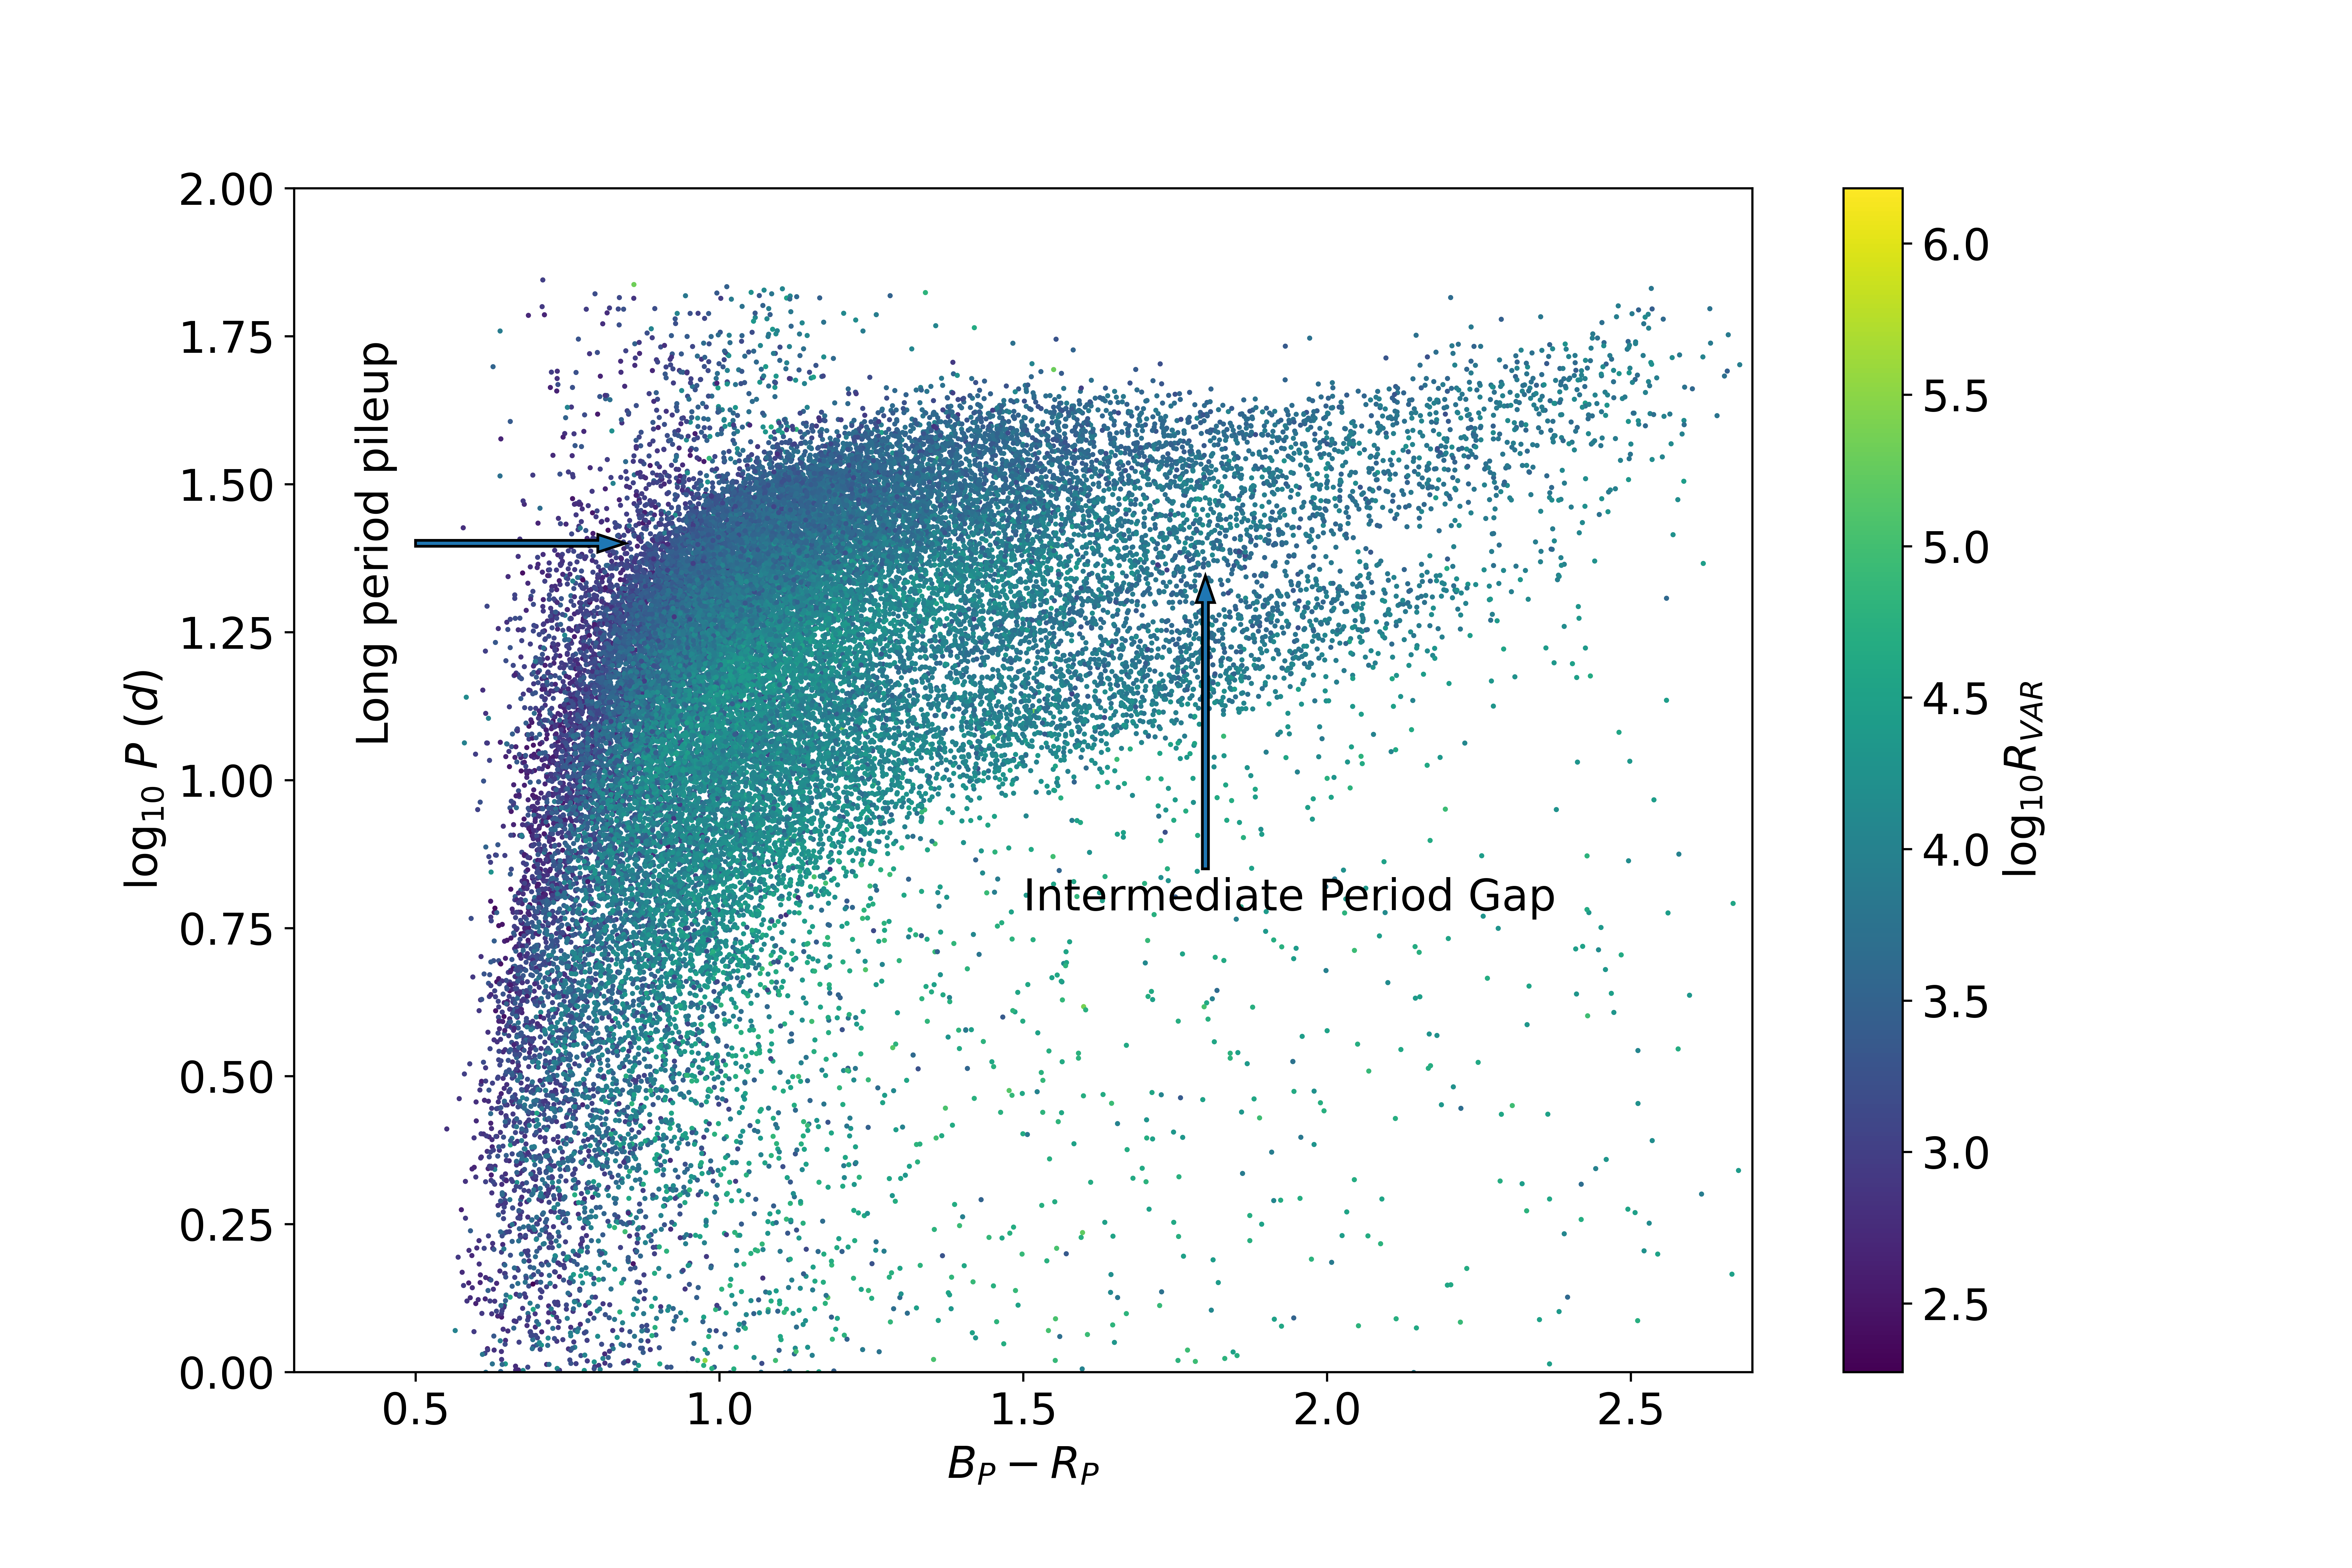
\includegraphics[width=\textwidth]{Figures/intro_figures/kepler_rot_dist.png}
    \caption[The rotational period distribution of the \citet{mcquillan_rotation_2014} sample featuring the intermediate period gap.]{A scatter plot showing \gaia{} $B_P-R_P$ colour against log of the \kepler{} \citet{mcquillan_rotation_2014} rotational period sample coloured by the log of the photometric variation ($R_{var}$).
    \update{$R_{var}$ decreases towards the gap from above and below, suggesting the gap is representative of a minimum of observability of rotation period. Highlighted by arrows in this figure are two features that we discuss in more detail in this section: the intermediate period gap and the long-period pile-up.}
    \todo{Improve visibility of the decrease of rvar}}
    \label{fig:kepler_rot_period}
\end{figure}


\update{Before exploring possible explanations for the gap, it is worth identifying where the rotational period gap occurs in the stars' evolution.}
\citet{reinhold_transition_2019} first suggested that the gap aligns with isochrone at $\sim$ 800 Myr using \citet{barnes_simple_2010} gyrochronological relations.
\update{\citep{reinhold_stellar_2020} updated this value to $\sim$ 750 Myr with a larger set of \ktoo{} data.}.
Contrary to the hypothesis that the gap aligns itself with a certain isochrone, \citet{curtis_when_2020} identified that the open cluster Ruprecht 147 contains stars above and below the gap, as well as one star that appeared to be within the gap.
This suggests that the gap does not align itself with a particular age.
Instead, they argued that the gap aligns itself with a line of constant Rossby number = 0.5.
\update{The Rossby Number is defined as the ratio of the rotational period to the convective turnover timescale ($R_{o} = P_{rot}/\tau_{conv}$) which itself is dependent on mass and is approximately constant for a star's main-sequence lifetime.}
The Rossby number is associated with the magnetic dynamo, \citep[see, e.g.,][]{noyes_rotation_1984, montesinos_new_2001, augustson_rossby_2019}
To simplify, a star can be thought of as a volume of charged particles.
As a star rotates, so do the charged particles within it.
Moving charged particles induce a magnetic field, creating a magnetic dynamo.
As the star rotationally evolves, so does the magnetic dynamo.

Given that the gap appears to line up with a line of constant Rossby number, this may suggest that the gap is instead caused by an event in the evolution of the magnetic dynamo rather than an event in time.
This is a notable result because the magnetic dynamo is associated with a number of stellar phenomena, such as magnetorotational instabilities (angular momentum transport processes associated with the magnetic field) or stellar spots.

Other prospective hypotheses for the intermediate period gap can be broken down into two categories: (1) bursty star formation, (2) modified angular momentum transport and (3) decreased observability of rotation periods.

\update{While the bursty star formation hypothesis is not a currently favoured hypothesis it led early studies into the intermediate period gap}
\citet{mcquillan_rotation_2014, davenport_rotating_2017} first proposed that the gap is the artifact of a recent period of bursty star formation in the \kepler{} field, resulting in a young ($<$ 50 Myr), fast rotating, population and older, background slowly rotating, population.
\citet{davenport_rotating_2017} \update{suggest} that the fast and slow rotators in this sample also exhibit a different distribution in proper motion. 
Two kinematically separate groups \update{would} favour the explanation of two epochs of star formation in the \kepler{} field. 
This explanation is further supported by the work of \citet{davenport_rotating_2018}, who \update{argued} that the observation of the gap correlates with Galactic height, which is assumed to be related to stellar age.

The recent bursty star formation hypothesis \update{would} account for the overpopulation of observations below the gap. 
In contrast, the dearth of observations represents the background observation rate of rotational periods within this period range.
\citet{gordon_stellar_2021} provided evidence against this hypothesis through analysis of \ktoo{} data.
They found that the intermediate period gap is present in the multiple pointings of the \ktoo{} mission - suggesting that recent bursty star formation is isotropic -  and that clusters with different ages contain stars that have crossed the gap.

The former suggests that\update{, for this hypothesis to be accurate,} all clusters universally went through a period of bursty star formation $\sim$50 Myr ago. 
\update{The two populations - above and below the gap - do not substantially universally differ in other spectroscopic and photometric observations.
This suggests that a universal two-population bursty star formation mechanism is not favoured.}
The latter requires slightly more thought. Comparing Figures \ref{fig:cluster_rotational_periods} and of \ref{fig:kepler_rot_period}, the gap has a sharper slope than the sequences associated with constant age populations from Praesepe \citep{douglas_poking_2017,douglas_k2_2019}, NGC 6811 \citep{curtis_temporary_2019} and Ruprecht 147 \citep{curtis_when_2020}. 
If the bimodal star formation scenario explained the gap, the gap should have the same shape and position for each cluster and the entire \ktoo/\kepler{} sample.


\update{Let us now consider that the gap results from modifications to angular momentum transport.
\citet{mcquillan_rotation_2014} first proposed that the gap is the result of two variations to Skaumanich rotational evolution.
They proposed that first, stars below the gap undergo a period of stalled spindown, resulting in the observed overdensity of stars along the lower branch, followed by a period of accelerated spindown, resulting in the dearth of stars in the gap.
For some time there was very little evidence nor a proposed mechanism for the period of accelerated spindown.}
Recent works by \citet{lu_bridging_2022} have shown that the gap is most apparent for stars less massive than 1.3 M$_{\odot}$ and more massive than 0.4 M$_{\odot}$.
If we look closely at Figure \ref{fig:ztf_comp} we can see that for the \ZTF{} sample (black dots) the intermediate period gap is most apparent for stars 1.5 $<B_P-R_P <$ 2.5 and closes for low mass ($B_P-R_P >$ 2.5) stars.
Stars redder than $B_P-R_P >$ 2.5 are fully convective \citep{amard_first_2019}, suggesting that the gap may be another phenomenon related to the interplay between angular momentum transport between the radiative core and convective surface and surface rotational braking along the main sequence.

\begin{figure}[h]
    \includegraphics[width=\textwidth]{Figures/intro_figures/ztf_comp.png}
    \caption[Rotation period distribution including fully convective stars.]{Rotation period against \gaia{} $B_P - R_P$ from \kepler{}, \ZTF{} overlayed with various open cluster measurements. Highlighted by this figure is the disappearance of the intermediate period gap above $B_P-R_P$ = 2.5 - the fully convective star boundary. This suggests that the rotational period gap is related to the coupling of the core and surface of low mass stars (0.4 $M_{\odot} <M< 1.3M_{\odot}$). Sourced from the top panel of Figure 8 in \citep{lu_bridging_2022}.}
    \label{fig:ztf_comp}
\end{figure}

The proposed mechanism underlying this scenario is the mass-dependent decoupling and recoupling of the core and the envelope proposed in 
\citet{lanzafame_rotational_2015} and \citet{spada_competing_2020}, discussed earlier in this work.
\citet{angus_exploring_2020} suggest that the core envelope decoupling and recoupling may explain the period gap as a break between a ``younger" pile-up regime ($R_o$ $<$ 0.6) in which surface rotation periods are relatively constant with time from core-surface angular momentum transport and increase with decreasing mass from an ``older" ($R_o$ $>$0.6) regime, with the gap representing a period of relatively fast spin evolution during the transition between the two.
Proponents of this hypothesis suggest that the gap results from a period of enhanced spindown following core and surface recoupling where stars ``jump" the gap before resuming Skumanich spindown, as is observed for older clusters.
Models of rotational evolution \update{(and the mechanism underlying the gap)} that reflect the proposed rapid spindown are yet to be identified.
Under this model, the gap reflects an under density of stars but would not be empty.
\update{A prediction of this model is that a non-zero population of stars will inhabit the gap.
\citet{curtis_when_2020} observed five Ruprecht 147 stars in or just beneath the gap that may express evidence of enhanced magnetic spindown, though these stars are yet to be thoroughly investigated.}

Now let us discuss the \update{final} catergory: the gap results from a lack of observations of rotational periods.
The rotational period of \kepler{} stars requires that stars express photometric oscillations from stellar spots.
Starspots are regions of intense magnetic activity on a star's surface from magnetic flux tubes in the convection zone. 
These flux tubes are thought to be stretched and curled by the differential rotation of the convective region. 
As a result, convection is inhibited, limiting plasma flow to the surface in these tubes.
This results in lower-temperature material within the tube, which looks like a darker spot on the star's surface.
Stellar spots have bright perimeters surrounding the cooler internal regions of spots, known as faculae.

Stellar spots can both increase or decrease stars' bolometric luminosity.
 \citet{reinhold_fast_2013} and \citet{reinhold_transition_2019} propose that the gap represents the transition in stellar spot structure from spot to faculae dominance in the photosphere.
Following their explanation, the gap corresponds to a transition where the increase in bolometric luminosity from the faculae negates the decrease from the internal, cooler region of the stellar spots. 
In the \citet{mcquillan_rotation_2014} sample, stellar rotational periods are measured from the period of brightness variability due to the brightness variability introduced by stellar spots\footnote{this technique is discussed in more detail in Section \ref{sec:techniques}}.
Suppose the bolometric flux does not vary due to stellar spots in the gap region. 
In that case, the amplitude of periodic variability would decrease within this region.
\citet{reinhold_transition_2019} suggests that the gap is full of stars and represents a minimum in the detectability of rotation periods.

Supporting this hypothesis, in both the \kepler{} and \ktoo{} fields, the variability amplitude ($R_{var}$) decreases towards the gap from both lower and higher rotational periods.
This can be seen in Figure \ref{fig:kepler_rot_period}, which is coloured by the log of $R_{var}$.
While there is evidence that stars undergo spot-to-faculae dominance, e.g. the Vaughan-Preston gap \citep{vaughan_survey_1980}, this occurs much later in a star's lifetime at $R_o$ $\sim$ 1.
Further, there is evidence that stars above and below the gap are both spot-dominated  \citep{lockwood_patterns_2007, reinhold_transition_2019}.
\citet{reinhold_transition_2019} speculate that activity cycles that vary the spot-to-faculae brightness contributions on rotational timescales could be the process underlying the rotational period gap.

Recent works have attempted to identify the fractional spot coverage of cluster members from their spectra \citep{cao_starspots_2022}.
They do this by assuming the spectra of stars can be broken down into spot and ambient components that vary in temperature but are consistent in other stellar parameters.
They find that the fractional spot coverage of stars is related to the Rossby number.
Within this work, they observe a population of spot-coverage-enhanced stars that deviate from the relations they present.

In a follow-up work \citep{cao_core-envelope_2023} they combine the angular momentum transport and decreased observation hypothesis by proposing
that star spot measurements in the Praesepe open cluster are strongly enhanced only for stars that depart Skumanich rotational evolution.
They suggest that a decoupling of the core and the surface explain both observations.
In their model, angular momentum transport between the core and the surface slows the increase of the rotational period. 
The resultant shears enhance the magnetic dynamo and, thus, stellar spot activity.
Stars enhanced in stellar spot coverage are expected to have decreased effective temperatures.
Spot-dominated, as opposed to faculae-dominated, stellar spots are cooler than the ambient temperature of the star.
As a result, stars with enhanced stellar spot coverage have a decreased observed effective temperature.
They then speculate that the rotational period gap is thus the result of a bias in observed effective temperature rather than a lack of observations of the rotational periods of stars in the gap.

Observations of open cluster rotational distributions beyond the gap suggest that stars $<1M_{\odot}$ that have crossed the gap ($R_o>$0.6) continue to spin down and follow the Skumanich-like rotational evolution until they leave the main sequence.
On the other hand, there is an apparent overabundance of stars at critical rotation periods (dependent on their mass). 
Above this is a lack of observations of rotation periods for stars $>$ 5500K.
Stars with higher masses also appear to have lower rotation periods on the pile-up than their less massive counterparts.
This results in what is known as the long-period pile-up, as noted in Figure \ref{fig:kepler_rot_period}.
The long-period pile-up aligns itself in the \citet{mcquillan_rotation_2014} period distribution with Rossby number  ($R_o$ = 2.08) \citep{van_saders_forward_2019}.
 
\citet{van_saders_forward_2019} suggest that the long-period pile-up could result from decreased magnetic braking or a lack of observations of stars beyond this Rossby number.
Under the former scenario, stars stop spinning down when they reach this Rossby number as a result of weakened magnetic braking.
This results in the overdensity of stars and a lack of observations of larger rotational periods.
In the latter, they propose that the error in observed periods can smooth out the overdensity of stars and, in fact the lack of rotational periods is because of variations to the stellar spot activity (See above discussion of speculative explanations for decreased observation of rotational periods within the rotational period gap).
Further supporting this explanation \citet{david_further_2022} found that photometric variability decreases above the gap.
\update{This suggests that there} is an unobserved population of stars with longer rotation periods.

Under the weakened magnetic braking model \citet{david_further_2022} suggest that stars $1M_{\odot} < M < 1.3M_{\odot}$ \update{in this temperature regime} may spend half of their main-sequence lifetimes at the long period pile-up with only modest variances to their rotational period.
Below this mass regime, stars appear to continue to lose angular momentum through wind braking following the Skumanich relation.
This results in stars with large rotational periods when they enter the post-main sequence.

%\todo write me
\update{\subsubsection*{Latitudinal differential rotation}}

%\update{Another facet of differential rotation is latitudinal rotation.
%This is the observation that the rotation profiles of stars differentially rotate dependent on latitude.
%As we touched on earlier this was first discovered in the Sun, where the equator was found to be rotating with a period of 25 days at the equator and 38 days at its poles.
%Within the surface convective envelope, the Sun is rotating equator-fast and has what is known as a solar-like rotation profile.
%The inverse of this is stars that are rotating with equator-slow latitudinal differential rotation profiles, known as anti-solar-like rotation profiles.
%Helioseismic measurements suggest that the surface latitude dependence of rotation disappears close to the base of the convective zone - however, these measurements become uncertain due to a decrease in the sensitivity of seismology internal to this point.
%However, the core of the Sun is thought to be solid-body rotating \citep{how_2009}.
%The internal latitudinal differential rotation of stars other than the Sun is currently unknown, but they are also thought to be solid-body rotating internal to the base of the convective zone.
%Therefore, throughout the rest of this Thesis, when we refer to latitudinal differential rotation we are referring purely to the surface latitudinal differential rotation.
%
%Rotating-magnetohydrodynamic models of stars \citep{brun_powering_2022} suggest that fast-rotating stars, $R_o\<0.5$ have latitudinally-flat or cylindrical rotation profiles, intermediate rotators, $0.5<R_o\< R_o_{\odot}$ have solar-like differential rotation profiles and stars where $R_o>2$ are anti-solar-like differentially rotating.
%The term "latitudinally flat" is a misnomer here.
%Observations suggest that very rapidly rotating stars ($R_o\< \< 0.5$) are consistent with latitudinal flatness. 
%However, differential rotation grows with $R_o$, and so "latitudinally flat" rotation profiles can, in fact, express equator-fast latitudinal dependence on rotation rate, the scale of the shear is just smaller than the arbitrary limit we place on what is considered to be "significant" latitudinal differential rotation.
%While \citet{benomar_asteroseismic_2018} found that, qualitatively, asteroseismic observations of the latitudinal differential rotation of solar analogues increase with $R_o$ and observations of young, fast-rotating stars with time-series doppler imaging are consistent with latitudinally flat differential rotation, observational confirmation of latitudinally flat or anti-solar-like differential rotation is yet to be made.

Another facet of differential rotation is latitudinal rotation.
This phenomenon refers to the observation that the rotation profiles of stars vary depending on their latitudes. 
This phenomenon was initially discovered in the Sun, where the equator completes a rotation in 25 days, while the poles take 38 days for a full rotation. 
Equator fast rotation of stars is described as solar-like differential rotation.
On the other hand, some stars exhibit equator-slow latitudinal differential rotation, known as anti-solar-like rotation profiles.
Helioseismic measurements indicate that this surface latitude dependence of rotation diminishes near the base of the convective zone, but measurements beyond this point become less reliable due to decreased sensitivity in seismology \citep{howe_solar_2009}.
While the internal latitudinal differential rotation of stars, apart from the Sun, remains unknown, it is believed that they also undergo solid-body rotation within the base of the convective zone. Hence, in this thesis, the term `latitudinal differential rotation' specifically pertains to surface latitudinal differential rotation.

Studies based on rotating-magnetohydrodynamic models of stars \citet{brun_powering_2022} suggest that stars with $R_o < 0.5$ tend to exhibit latitudinally-flat, or perhaps, cylindrical rotation profiles.
Intermediate rotators ($0.5<R_o< R_{o \ \odot}$) have solar-like differential rotation profiles, while stars where $R_o>2$ are thought to exhibit anti-solar-like rotation profiles.
However, it's worth noting that the term `latitudinally flat' is somewhat misleading. 
Observations indicate that very rapidly rotating stars ($R_o < 0.5$) in fact, express equator-fast latitudinal dependence on rotation rate, with the scale of the shear being just smaller than the arbitrary limit set for considering it as `significant' latitudinal differential rotation.
Recent studies by \citet{benomar_asteroseismic_2018} suggest that observations of the latitudinal differential rotation of solar analogues increase with $R_o$, while observations of young, fast-rotating stars using time-series Doppler imaging are consistent with latitudinally flat differential rotation. 
However, definitive observational evidence confirming latitudinally flat or anti-solar-like differential rotation is yet to be established.
The post-main sequence evolution of latitudinal differential rotation is also a currently unexplored field of study.
We do not know if post-main sequence stars do express latitudinal differential rotation nor if they are expected to theoretically.


%Theoretical work on the mechanisms underlying differential rotation is an ongoing field.
%In the surface convective region of low-mass stars, angular momentum is believed to be redistributed in four ways.
%Meridional circulation, which flows in the radial and latitudinal direction, convective flow in the radial direction, magnetic forces, and viscous diffusion.
%The position and strength of each of these mechanisms are currently uncertain and require further work to determine their effect on the evolution of latitudinal differential rotation.}
%
%Our understanding of the evolution of latitudinal differential rotation in low-mass stars is limited.
%Current techniques are either inaccurate, imprecise or limited to certain stars making inference of the evolution of differential rotation difficult.
%Here we will outline those techniques and their limitations.
%Early works focused on the effect of stellar spots spectral line features - Doppler imaging.
%The presence of spots on the surface of a star creates perturbations on the spectroscopic line profile, dependent on the position of the spot.
%Time-series Doppler imaging is able to gauge the rotation rate at different latitudes and thus the surface differential rotation can be measured.
%This method is limited in use due to the necessity of high-cadence long baseline time-series spectroscopy.
%Furthermore, surface features and their position on the surfaces of stars can be degenerate in such a method.
%\citet{collier_2007} suggests that the errors associated with this method are often underestimated.



The study of the mechanisms behind differential rotation remains an active and ongoing field of research. 
In the surface convective region of low-mass stars, there are four believed mechanisms responsible for redistributing angular momentum: latitudinal and radial flows from meridional circulation, convective flow in the radial direction, magnetic forces, and viscous diffusion. 
The exact positions in the convective region and relative strengths of these mechanisms are currently uncertain and require further investigation to understand their impact on the evolution of latitudinal differential rotation.

Unfortunately, our understanding of the evolution of latitudinal differential rotation in low-mass stars is still limited, primarily due to the shortcomings of the current techniques used for analysis. These methods often suffer from inaccuracies, lack precision, or are applicable only to specific stars, making it challenging to infer the evolution of differential rotation accurately.

One of the early techniques used in this research involved studying the effect of stellar spots on spectral line features, known as Doppler imaging. 
By observing the perturbations caused by spots on the spectroscopic line profile and analysing the position of these spots, researchers could estimate the rotation rate at different latitudes and thereby measure the surface differential rotation. However, this method has its limitations. It requires high-cadence long baseline time-series spectroscopy, which may not always be readily available. Additionally, the interpretation of surface features and their positions on stars can be ambiguous, leading to potential degeneracy in the results. 
It is worth noting that \citet{collier_differential_2007} has raised concerns about underestimated errors associated with this method.

\citet{reiners_rotation_2002}, on the other hand, developed a Fourier-transform-based method to determine latitudinal differential rotation from a single observation of the spectroscopic line shape.
The method uses the deviation of line profiles from a rigidly rotating surface to estimate the latitudinal differential rotation.
While the benefit of requiring a single spectroscopic observation of a star is obvious, the applicability is limited.
The method is limited to magnetically active fast rotators (\vsini $\>$ 10km/s), where line-broadenings are large enough to be well resolved.
\citet{barnes_dependence_2005, reiners_rotation_2002} adopt this method and confirm that latitudinal differential rotation increases with increasing temperature for young, rapidly rotating, magnetically active stars.
The observation of differential rotation using this method is limited to young stars - the evolution of differential rotation with age cannot be probed using this method.

Another prospect for measuring differential rotation arises through the latitudinal variation in the position of stellar spots and thus the measurement of multiple periods in a light curve (\citep[see, e.g.,][]{walcowicz_rotation_2013, reinhold_rotation_2013}.
Measuring latitudinal differential rotation in this way is straightforward in theory.
If multiple surface features appear at different latitudes then multiple peaks in the power spectrum arise from which the different rotation periods can be measured.
The difference between the two periods provides a measure of the surface rotational shear.
The latitudes at which the surface features arise cannot be probed using this method and the distribution of stellar spots on the surface of a star is unknown.
Therefore, the surface rotation profile cannot be probed.

If surface rotational shear is relatively small, as it is for say the Sun, then latitudinal differential rotation then the power spectrum of the light curve would contain closely space peaks that can appear as a single broad peak in real data.
The broadness of a feature in Fourier space is also related to the lifetime of that feature in period space.
Because of this, the inference of latitudinal shear from time series integrated photometry is limited.
\citet{aigrain_hare_2015} compared methods of measuring rotational period and latitudinal shear using synthetic \kepler\ data.
They found that no state-of-the-art method \citep[e.g., those adopted by ][]{reinhold_rotation_2013, mcquillan_rotation_2014, garcia_rotation_2014} are able to disentangle the effects of latitudinal differential rotation from the surface feature lifetime.
Surface differential rotation cannot be accurately measured through this method

Asteroseismic inversions of latitudinal differential rotation prove to be somewhat fruitful in measuring the evolution of latitudinal differential rotation.
\citet{benomar_asteroseismic_2018, bazot_latitudinal_2019, hall_weakened_2021} were able to perform inversions of the rotational splittings of main-sequence stars using \kepler\ data.
Their combined sample includes 14 stars with significant detection of solar-like differential rotation.
They also report a number of other stars investigated in their work show limited evidence of solar-like and anti-solar-like latitudinal rotation.
The significance of detection is related to the scale of the latitudinal shear.
This complicates the inference of the evolution of latitudinally flat and anti-solar-like differential rotation profiles which tend to express small scales of latitudinal shear,
Further, their investigations are limited to a small number of stars that have long-baseline time-series photometric observations that express solar-like oscillations below the Nyquist frequency of \kepler{}.
This limits our understanding to, essentially, solar analogues.

\subsection{Post-main sequence}

For low mass (1.1 - 1.5 M$_{\odot}$) stars during the post-main sequence, \update{angular momentum transport between the core and the surface can be probed.}
While surface rotation can still be measured through stellar spot photometric oscillations, within this regime, the core and surface can also be simultaneously constrained through asteroseismology (at different points in evolution). 
\update{This results from a combination of the expression of mixed modes, shorter mode lifetimes, and increased core rotation rates.
We can separate the observed modes of stars into distinct flavours: pressure (p) modes, gravity (g) modes, and mixed modes.
p and g modes correspond to oscillations propagating in the convective envelope, and the result of trapping of gravity waves in the radiative core with buoyancy as a restoring force, respectively. 
During the main sequence, g-modes are trapped within the radiative core and thus do not introduce brightness variations (oscillations) to the stellar surface
Some g-modes can couple with p-modes in the surface convective cavity during the post-main sequence and are known as ``mixed modes".
The rotational splittings of the mixed modes allow us to infer the rotation rate in the radiative region and deep core \citep{metcalfe_precise_2010,bedding_gravity_2011}.
Where, precisely, the mixed modes probe is dependent on where in the post-main sequence the star is observed.
For example, sub-giant stars express p-modes and mixed modes that can probe both the core and the surface, whereas red giant branch (RGB) stars mainly express mixed modes that can only probe the star's core.
While stellar spot surface rotation periods can be measured for post-main sequence stars \citep{mcquillan_rotation_2014, ceillier_surface_2017}, asteroseismic inference of core and surface rates is the standard for probing rotation evolution in this regime \citep{deheuvels_seismic_2014, gehan_core_2018, deheuvels_seismic_2020, fellay_asteroseismology_2021}.}

Measuring the core and surface rotation rates simultaneously provides much more information to angular momentum transport than either of these quantities alone.
For example, during the main sequence, the over-abundance of stars along the lower branch of the \update{\kepler{}} rotation period gap could simultaneously be explained by diminished wind braking for the surface or by core-envelope recoupling.
Measuring the core rotation rates would break this degeneracy.
This asteroseismic quirk is useful as it allows us to directly investigate angular momentum transport more efficiently.

However, the constraints to the rotation profile of stars by asteroseismology, even in the post-main sequence, are limited.
The core and surface rotation rates of subgiants can simultaneously be probed.
However, where in a star the rotation can be probed depends on the observed oscillation modes, which depend on the stellar structure.
The rotation rates obtained by asteroseismology are kernel-based averages of the rotation profile in regions that the observed oscillation modes probe.
For example, subgiants' core and surface rotation rates are the kernel-based average rotation rates of the innermost $r/R<0.05$ and outermost $r/R>0.9$ regions (on average).
Between these regions, the rotation profile is not constrained.
As a result, the shape of the rotation profile, which can be fingerprints of specific angular momentum transport mechanisms at play, is also not constrained.

Asteroseismic inference of rotation rates can also be imprecise.
This can be seen when comparing the surface rotation periods from asteroseismology and stellar spot photometric oscillations in \citet{hall_weakened_2021}.
This is because: a) state-of-the-art measurements of rotational splittings - the quantity that constrains the rotation profile - are low SNR and are often also imprecise, and b) the observed rotational splittings are a finite subset of the infinite number of rotational splittings that would be required to accurately and precisely constrain the entire rotation profile.
With these limitations in mind, we now discuss the observed evolution of rotation of post-main sequence stars.

Following the main sequence, low-mass stellar rotation varies with the evolutionary phase.
Models of rotating stellar evolution \citep[see, e.g.,][]{maeder_evolution_2000,heger_presupernova_2000} predict the following qualitative evolutionary pathway.
Towards the end of the main sequence the rotation profile is largely flat.
Assuming conservation of angular momentum as hydrogen core burning stops, pressure in the core drops, resulting in core contraction while the convective surface region expands.
Resultingly the core is spun-up while the surface is spun-down.
The core should continue to spin up as the core contracts along the RGB until entering the red clump (low-mass core He burning).
The core burning reintroduces core pressure, and the resulting expansion of the core decreases the core rotation rate.
When core He burning ceases, the core pressure drops again, resulting in a spun-up white dwarf (relative to the core rotation rate of red clump stars).
We highlight the qualitative rotation evolution of post-main sequence stars in Figure \ref{fig:poms_evo}.
Observations suggest that low-mass stars follow this pathway \citep{mosser_spin_2012,deheuvels_seismic_2014,deheuvels_seismic_2015,hermes_white_2017,gehan_core_2018,deheuvels_seismic_2020}.

\begin{figure}[h]
    \includegraphics[width=\textwidth]{Figures/intro_figures/qualitative_evo.png}
    \caption[Qualitative core and surface rotation rates of post-main sequence stars.]{Core (red) and surface (blue) rotation rates with additional angular momentum transport following the prescription of \citet{spada_angular_2016}. Coloured sections denote evolutionary milestones and the works that have provided constraints to these milestones. \textbf{Pink:} subgiant core and surface rotation, \textbf{Orange:} red giant branch cores, \textbf{Green:} clump core rotation rates, and \textbf{Purple:} white dwarf rotation rates. Adapted from Figure 3 in \citet{fuller_slowing_2019}}
    \label{fig:poms_evo}
\end{figure}


Measuring the core and the surface rotation rates of post-main sequence stars allows us to place constraints on the radial differential rotation of stellar interiors and quantitatively probe the evolution of angular momentum transport.
Observations of young subgiants suggest that terminal age main sequence stars' rotation profiles are relatively flat \citep{deheuvels_seismic_2020}.
However, observations of older post-main sequence stars have raised more questions than they have answered \citep{beck_fast_2012}.
To summarise: angular momentum transport during the post-main sequence must be greater than state-of-the-art models currently predict.

\citet{deheuvels_seismic_2014} measured the core and surface rotation rates of 6 subgiants/young red giants.
The observed core to surface rotation ratio of subgiants and the core rotation rates of red giant branch stars suggest that additional angular momentum transport is unaccounted for in state-of-the-art models of rotating stellar evolution \citep{deheuvels_seismic_2014, spada_angular_2016, moyano_asteroseismology_2022}.
The scale of the core-to-surface rotation rate ratio of subgiants ($\Omega_c / \Omega_s$) is one to two orders of magnitude smaller than models predict \citep{fuller_asteroseismology_2015,spada_angular_2016,ouazzani_gamma_2018, eggenberger_asteroseismology_2019}.
While core rotation rates were first believed to decrease along the red giant branch\footnote{Indeed when core rotation rates of red giants are plotted against $\log{g}$, a proxy for evolution, they do appear to decrease with evolution. When plotted against the more appropriate scale of mixed mode coupling (see Equation 10 in \citet{gehan_core_2018} and compare Figures 12 and 13 in this work), they are constant with evolution.} \citep{mosser_spin_2012} revised measurements and a larger sample size revealed that the core rotation rates of red giant branch stars appear constant with evolution when the contraction of the core should spin them up.
\citep{mosser_spin_2012,gehan_core_2018,moyano_asteroseismology_2022}.
The core rotation rates of early red giant branch and red clump stars suggest a continued excess angular momentum transport during this phase of evolution \citep{cantiello_angular_2014,moyano_asteroseismology_2022}.
On the other hand, observed white dwarf rotation rates can be recovered from the observed core rotation of clump stars assuming conservation of angular momentum \citep{cantiello_angular_2014, den_hartogh_constraining_2019}.
\citet{cantiello_angular_2014} suggests that this feature may be owing to the short evolutionary timescale between the red clump and white dwarf phases rather than indicative of a decrease in the excess angular momentum transport.


The physical mechanism underlying the excess angular momentum transport is currently unidentified.
Several notable relations with mass and evolutionary state have been determined by calculating the excess angular momentum transport required to match observations. 
\citet{spada_angular_2016} quantified the increased angular momentum transport required to match the observed subgiant core and surface rotation rates measured in \citet{deheuvels_seismic_2014}.
They introduced an additive angular momentum diffusion coefficient to the transport of angular momentum equation in the radiative zone, which obeys an advection-diffusion equation \update{\citep{zahn_circulation_1992,maeder_stellar_1998,eggenberger_geneva_2008} }
\begin{equation}
    \rho \frac{\text{d}}{\text{dt}}\left(r^2 \Omega \left( r \right)\right) = \frac{1}{5r^2}\frac{\partial}{\partial r}\left(\rho r^4 \Omega \left( r \right)
 \ U\left(r\right)\right) + \frac{1}{r^2}\frac{\partial}{\partial r} \left(\rho \left( D_{\text{shear}} + v_{\text{add}}\right) r^4 \frac{\partial \Omega\left( r \right)}{\partial r}\right),
\end{equation}
where $r$ and $\rho$ are the characteristic radius and density on an isobar. $\Omega(r)$ is the mean rotational rate and $U(r)$ is the velocity of meridional currents in the radial direction. $D_{\text{shear}}$ is the diffusion coefficient for the angular momentum shear instability (see Equation 10 in \citet{eggenberger_effects_2010}) and $v_{\text{add}}$ is the additional viscosity corresponding to the excess angular momentum transport.
Their results suggest that the additional angular momentum transport decreases as stars ascend the subgiant branch and increases with mass.
The suggested scale of excess angular momentum transport they propose is on the order of \update{$10^3-10^4 \ \text{cm}^2 \text{s}^{-1}$}.
Which is similar to $D_{\text{shear}}$ close to the convective envelope but rapidly decreases to the order of \update{$10^1\ \text{cm}^2 \text{s}^{-1}$} in the stellar core.
Comparing Figures \ref{fig:deh_without} and \ref{fig:deh_with} we see that the introduction of additional viscosity to the model term results in agreement with the core to surface rotation fraction in the \citet{deheuvels_seismic_2014} sample.

\citet{moyano_asteroseismology_2022} performed a similar analysis but with the core rotation rates of red giant branch and red clump stars measured in \citet{mosser_spin_2012} and \citet{gehan_core_2018}.
They found that the same order of magnitude additional viscosity term was required to explain the approximately constant core rotation rates of red giant and red clump stars.  
Qualitatively they found that the additional angular momentum transport becomes stronger when the star evolves up the red giant branch through shell hydrogen burning.
Angular momentum must be redistributed between two to three orders of
magnitude more efficiently for red clump stars than for red giants closer to the main sequence turn-off, consistent with \citet{den_hartogh_constraining_2019}.
Figures \ref{fig:deh_with} and \ref{fig:rgb_cores_without}  highlight that models of red-giant evolution with the additional viscosity introduced in this work now agree with the observed core rotation rates observed in \citet{gehan_core_2018}.

\begin{figure}[h]
    \includegraphics[width=\textwidth]{Figures/intro_figures/deheuvels_disparity_without.png}
    \caption[A comparison of modelled and observed core to surface rotation rate ratios of post-main sequence stars without additional angular momentum transport.]{Logarithm of core to surface rotation rate against stellar surface gravity. 
    \textbf{Dots:} Observed core to surface rotation rates of the six subgiants measured in the \citet{deheuvels_seismic_2014} sample (A,B,C,D,E,F).
    \textbf{Lines:} rotating models of the stars in that sample without additional angular momentum transport \citep{eggenberger_asteroseismology_2019}.
    The observed core-to-surface rotation rates are much smaller than models predict. This implies additional angular momentum transport than is currently accounted for models.
    Sourced from Figure 2 in \citep{eggenberger_asteroseismology_2019}.}
    \label{fig:deh_without}
\end{figure}

\begin{figure}[h]
    \includegraphics[width=\textwidth]{Figures/intro_figures/deheuvels_disparity_with.png}
    \caption[A comparison of modelled and observed core to surface rotation rate ratios of post-main sequence stars with additional angular momentum transport.]{Same as Figure \ref{fig:deh_without} but with additional angular momentum transport introduced for the models to reflect the observations.
    Sourced from Figure 3 in \citep{eggenberger_asteroseismology_2019}.}
    \label{fig:deh_with}
\end{figure}


\begin{figure}[h]
    \includegraphics[width=\textwidth]{Figures/intro_figures/rgb_core_rot_without.png}
    \caption[Average core rotation rates of red giants against mixed mode density without additional angular momentum transport]{Average core rotation rates of red giants against mixed mode density (a proxy for evolution).
    \textbf{Dots:} Observed core rotation rates from \citet{gehan_core_2018}
    \textbf{Lines:} rotating models of the stars in that sample without additional angular momentum transport \citep{moyano_asteroseismology_2022}.
    The observed core rates are much smaller than models predict, implying excess angular momentum transport is required for the models to reflect the observations.
    Sourced from Figure 6 in \citep{moyano_asteroseismology_2022}.}
    \label{fig:rgb_cores_without}
\end{figure}

\begin{figure}[h]
    \includegraphics[width=\textwidth]{Figures/intro_figures/rgb_core_rot.png}
    \caption[Average core rotation rates of red giants against mixed mode density without additional angular momentum transport]{Same as Figure \ref{fig:rgb_cores_without} but with additional angular momentum transport introduced for the models to reflect the observations.
    Sourced from Figure 7 in \citep{moyano_asteroseismology_2022}.}
    \label{fig:rgb_cores_with}
\end{figure}


Several modes of excess angular momentum transport have been suggested to explain the disparity between models and observations.
\citet{barker_angular_2019,barker_angular_2020} studied the role of
the Goldreich-Schuber-Fricke (GSF) instability \citep{goldreich_differential_1967,fricke_rotation_1967} and its role in angular momentum transport for post-main sequence stars.
They suggest that the GSF instability can introduce additional viscosity up to $10^4 \ \text{cm}^2 \text{s}^{-1}$ for low-mass stars but is two orders of magnitude too small to reflect the rotation of higher mass stars not discussed in this work.

Magnetorotational instabilities constitute another candidate to explain the internal rotation of evolved stars.
Two potential candidates are azimuthal magnetic rotational instabilities \update{\citep[AMRI; see ][]{ruediger_astrophysical_2014,rudiger_diffusive_2015}} and the Tayler-Spruit instability \citep[see ][]{spruit_dynamo_2002}).
\citet{rudiger_diffusive_2015} suggest AMRIs can increase molecular viscosity to the magnitude required to explain observations.
On the other hand, there is no evidence to suggest that this instability reflects the trends with mass and evolution.
The Tayler-Spruit instability does introduce excess angular momentum transport in the post-main sequence \citep{fuller_slowing_2019}, however, it cannot simultaneously reflect the observations of both subgiants and red giants \citep{eggenberger_asteroseismology_2019,den_hartogh_constraining_2019}.


\citet{spada_angular_2016} propose the efficiency of angular momentum transport may be related to the core to surface rotation rate to some power - $\left(\Omega_c/\Omega_s\right)^{\alpha}$ - which can be related to magnetorotational instabilities.
This work suggests that an $\alpha$ of reflects the core rotation rates of red giants claimed in \citet{mosser_spin_2012}.
\citet{moyano_asteroseismology_2022} revisited this prescription and found that $\alpha = 3$ more accurately reflects the approximately constant rotation core rotation rates of red giants observed by \citet{gehan_core_2018}.
\citet{spada_angular_2016} was limited to a single model with a mass of 1.25 $M_{\odot}$.
No parameterisation with mass was therefore performed.

Other physical mechanisms have been suggested to have a role in excess angular momentum transport, such as angular momentum transport by internal gravity waves \citep{pincon_can_2017} or mixed-modes \citep{belkacem_angular_2015}. 
However, the scale of their introduced additional viscosity is yet to be investigated.
Disentangling each of these proposed mechanisms' relative importance to the additional angular momentum transport required to explain the observations requires much more data.


%On the other hand the subgiant phase is short-lived and steroseismic inference of the rotation profile is data-intensive in that it requires short-cadence observations of stars over long observation periods for high enough SNR to measure rotational splittings.
%As a result, only ~30 subgiant and young red giants that exhibit oscillation modes that probe both the core and the surface have been asteroseismically probed.

We speculate that the simultaneous measurement of subgiants' core and surface rotation rates may be the best probes for constraining the excess angular momentum transport.
A few pathways exist to further probe the mechanism underlying excess angular momentum transport through asteroseismology alone.
\update{Either more stars need to have their core and surface rotation rates measured through asteroseismology (which we will denote ensemble fitting), or stronger constraints must be placed on the rotation profile between the core and the surface (single star constraints).}

If more stars have their core and surface rotation rates observed, then more measurements of the excess angular momentum are required for state-of-the-art models to match.
The excess angular momentum transport required to match observations appears to \update{depend on mass and evolution}.
Stronger constraints on the dependency of the excess angular momentum transport on these quantities provide information about the underlying mechanism.
The Kepler asteroseismic data currently available suggests that the efficiency of the excess angular momentum transport increases with the star's mass \citep{eggenberger_asteroseismology_2019}.
However, the efficiency of angular momentum transport decreases with evolution during the subgiant phase.
Consequently, a transport process with efficiency dependent on the angular momentum gradient between the core and the surface cannot be at play in subgiants.
Identifying with more precision the dependency of excess angular momentum transport on stellar quantities would provide evidence for or discredit proposed mechanisms.

\update{The internal shape of the rotation profile of subgiants reflects the underlying mechanism that created it.}
Therefore, evidence for or against particular shape of rotation profiles is illuminating to proposed mechanisms.
A strong gradient in the rotation profile in the core of a subgiant, for example, is incompatible with angular momentum transport through deep fossil magnetic fields \citep{gough_effect_1990} as they would likely smooth out sharp features.
 This is because differential rotation is expected to be damped along poloidal field lines (\citealp{garaud_rotationally_2002, strugarek_magnetic_2011}).
 Internal gravity waves, on the other hand, are expected to be efficient during the advanced phases of stellar evolution \citep{charbonnel_deep_2008}. 
Internal gravity waves can give birth to localised weak gradients in the rotation profile as a result of extraction and deposit of angular momentum \citep{charbonnel_influence_2005}. 
A sharp rotational gradient could also potentially trigger magneto-rotational instabilities that would transport angular momentum (\citealp{balbus_stability_1994,arlt_differential_2003,menou_magnetorotational_2006, fuller_asteroseismology_2015, fuller_slowing_2019,moyano_asteroseismology_2022}). 
Evidence of a strong angular momentum gradient towards the core of a sub-giants quickly constrains the number of possible angular momentum transport mechanisms to solve the angular momentum transport problem.

Two obvious problems impede the single-star pathway. 
These are the need for observations of high SNR higher degree modes and the results of methods used to measure rotation profiles being unstable to high-resolution inversions. 
Constraints on the rotation profile in intermediate points between the core and surface require the observations of oscillation modes of $l \approx 10$ \citep{ahlborn_asteroseismic_2020}. 
For reliable measurements of such oscillations, much longer observation periods, longer than \corot{} and \kepler{}, of sub-giants are required.
   
Both of these pathways require much more asteroseismic data than is currently available.
For ensemble fitting to be viable many subgiants would need to be observed over long baselines with short cadence observations.
If the \kepler{} mission is exemplary, then the baseline required for high-SNR asteroseismic observations is on the order of ~4 years per star.

At the time of writing, \update{of order thirty} subgiants show evidence of rotational splittings \citep{li_asteroseismology_2020,li_asteroseismology_2020-1}, though the rotational splitting data is yet to be released and analysed.
The results will be undoubtedly informative, though we will not speculate exactly how much they will solve the subgiant excess angular momentum transport problem.
\citet{hatt_catalogue_2023} suggests that there are \update{of order four thousand} stars in the \tess{} - short cadence catalogue with observable solar-like oscillation features.
The measured frequency of peak oscillation power $\nu_{\text{max}}$ of stars in these sample suggests that some of these stars are subgiants.
While no rotational splittings of these stars have been reported, some of these stars may lay in the continuous viewing zone.
This means their observation periods are approaching 4 years at time of writing and these stars may soon offer a seperate sample of subgiants with observations of asteroseismic rotational splittings.
While we may speculate about future asteroseismic focussed missions, it will be some time before any new asteroseismic rotation signals in subgiants are made.

Independent constraints can also be placed on the evolution of the surface rotation of subgiants.
\citet{santos_surface_2021} measured the surface rotation of \update{four thousand five hundred} subgiants using photometric oscillations from stellar spots.
The measured rotational periods against their effective temperature are shown in Figure \ref{fig:subgiant_surface}.
Within this figure, there are a few notable features.
While subgiants are definitionally older than their main-sequence counterparts, there is a sample of fast-rotating stars coincident with the fast rotators on the main sequence.
This could be explained by most of the stars in this sample being a higher mass than the Kraft break.
They have passed through the main sequence with fast rotating surfaces, entering the subgiant phase; their effective temperatures decrease and are shifted to the right in this diagram relative to their main-sequence counterparts.
The high density of fast-rotating stars could also result from an observational bias.
Long rotational periods require longer baselines to recover and thus have a decreased observed fraction.
Among the sample is a group of slow-rotating (period $>$ 60 days) targets with \teff{} between 5000 and 6000 K.
These are consistent with more evolved subgiants as the slowest of these targets are located close to the red giant branch.
This work also suggests that the decreased observation of rotation periods $>$60 days, the strong upper edge of the \citet{mcquillan_rotation_2014} rotational period distribution, is the result of a lack of observations of main-sequence stars rather than an inherent lack of long period probing power by \kepler. 
Whether the upper edge results from angular momentum transport or decreased photometric variability is unknown.
The final feature that is not commented on in their work is an apparent dearth of observations coincident with the intermediate period gap.
Whether this is real or a result of noise is an interesting avenue of research in further understanding the underlying mechanism of the intermediate period gap for main-sequence stars.

\begin{figure}[h]
    \includegraphics[width=\textwidth]{Figures/intro_figures/subgiant_surface.png}
    \caption[Surface rotation period distribution of subgiant stars]{Surface rotation period against effective temperature of subgiants in the \citet{santos_surface_2021} sample overlayed over the \kepler{} \citet{mcquillan_rotation_2014} sample. 
    Sourced from the bottom panel of Figure 5 in \citep{santos_surface_2021}.}
    \label{fig:subgiant_surface}
\end{figure}

\citet{ceillier_surface_2017} measured the surface rotation periods of 361 red giants from stellar spot photometric variability.
The measured rotational periods against their mass are shown in Figure \ref{fig:rgb_surface}.
Expectedly, compared to the subgiant analysis of \citet{santos_surface_2021} the surface rotation period of red giant stars is greater than their subgiant counterparts.
They suggest that the surfaces of these stars rotate faster than models suggest \citep{tayar_rapid_2015}.
They conclude that the large percentage of rapid rotators must result from interactions of red giants with other bodies.
This work, however, is older than the revised excess angular momentum transport research discussed earlier in this work.
Their results need to be reexamined within the context of excess angular momentum transport.

\begin{figure}[h]
    \includegraphics[width=\textwidth]{Figures/intro_figures/rgb_surface.png}
    \caption[Surface rotation period distribution of red giant stars]{Surface rotation period against mass of red giant stars from \citet{ceillier_surface_2017}.
    Sourced from the top panel of Figure 7 in \citep{ceillier_surface_2017}.}
    \label{fig:rgb_surface}
\end{figure}

Finally, we discuss the rotating remnants of low-mass post-main sequence evolution: white dwarfs.
White dwarfs do not evolve rotationally, though their observed rotation rates constrain angular momentum during the red clump phase.
\citet{hermes_white_2017} suggest that the rotation periods of white dwarfs decrease with the progenitor's mass.
As previously discussed, the surface rotation rates of white dwarfs are consistent with angular momentum conservation following the red clump \citep{den_hartogh_constraining_2019, cantiello_angular_2014}.
This is because the time scale of angular momentum transport is longer than the timescale of evolution from red clump star to a white dwarf.
\citet{den_hartogh_constraining_2019} suggest that mass-dependent angular momentum transport must decrease with evolution along the red clump such that the angular momentum of terminal red clump rotation cores agree with the angular momentum of white dwarf stars.

\subsection{Effects of rotation on low-mass evolution}
\label{sec:effects}

In this Section, we will summarise the observable features of rotation on low-mass stellar evolution.
Compared to high-mass rotating stellar evolution, the indicators of low-mass rotating stellar evolution are minimal \citep[see, e.g.,][]{heger_presupernova_2000, maeder_evolution_2000}.
The rotation rate is the main observable property of the evolution of rotation in stars.
As this was discussed in length in Section \ref{sec:evolution} we will focus here on the impact of rotation on other observable quantities and a star's evolution.

\begin{figure}[h]
    \includegraphics[width=\textwidth]{Figures/intro_figures/PMS_effect.png}
    \caption[Effect of rotation on pre-main-sequence evolution of a 1 $M_{\odot}$ star.]{Effect of rotation on post-main-sequence evolution of stars. Left: PMS HR diagram tracks of 1 M$_{\odot}$ solar metallicity models with and without rotation. The continuous line corresponds to a non-rotating model, while the dashed line corresponds to a rotating model with $\Omega = 20 \Omega_{\odot}$. The tracks end when the ZAMS is reached. Right: Surface lithium abundance with time during the PMS for the same models. Sourced from Figure 1 in \citet{eggenberger_rotation_2013}}
    \label{fig:pms_effect}
\end{figure}

Figure \ref{fig:pms_effect} (left) compares the evolutionary track of a rotating solar-type, 1M$_{\odot}$, solar metallicity, star rotating with 20 $\Omega_{\odot}$ (twenty times the mean solar surface rotation rate) against a non-rotating model of the same mass and metallicity. 
Because of the introduction of the centrifugal force, the HR path is slightly shifted towards lower effective temperatures and luminosities than a non-rotating star.

During the pre-main sequence, both the changes to the rotation impact the observed lithium abundances, which are dependent on the treatment of angular momentum transport \citep{dumont_lithium_2021}.
Figure \ref{fig:pms_effect} (right) displays the evolution of surface lithium abundance during the PMS phase for rotating and non-rotating models. 
The zero-age-main-sequence (ZAMS) surface lithium abundance of the rotating model is lower than that of the non-rotating model, indicating that including rotational effects increases lithium depletion during the PMS. 
However, during the beginning of the lithium depletion phase, the rotating model shows a slightly higher lithium content than the non-rotating one due to the centrifugal force lowering the temperature at the base of the convective envelope.

As the star develops a radiative zone at its centre, rotational mixing becomes the dominant factor in transporting lithium to deeper and hotter regions, where it is efficiently destroyed. 
This leads to a lower surface lithium abundance for the rotating model on the ZAMS compared to the non-rotating model due to the increase in differential rotation in the stellar interior during the PMS.

The duration of the disc-locking phase, which enhances differential rotation in the radiative zone, significantly impacts the sensitivity of the lithium content in rotating models. 
Longer disc lifetimes lead to lower surface lithium abundances on the ZAMS due to increased angular velocity gradients below the convective envelope, which enhance rotational mixing \citep{eggenberger_angular_2012}. 
Moreover, as the star loses more angular momentum during the longer disc-locking phase, it reaches the ZAMS with a lower surface rotational velocity, resulting in lower lithium abundance.
Therefore, a correlation between the surface velocity and lithium abundance on the ZAMS exists: stars with lower rotation rates on the ZAMS are expected to be more depleted in lithium than fast rotators on the ZAMS.

\begin{figure}[h]
    \includegraphics[width=\textwidth]{Figures/intro_figures/MS_effect.png}
    \caption[Effect of rotation of main-sequence evoltuon of a stars 1 $M_{\odot}$]{Left: MS HR diagram tracks of 1 M$_{\odot}$ solar metallicity models with and without rotation. The continuous line corresponds to a non-rotating model, while the dashed line corresponds to a rotating model with ZAMS surface velocity = 50 km/s. The tracks end when the ZAMS is reached. Right: Surface helium abundance with time during the MS for the same models. Sourced from Figure 3 in \citet{eggenberger_rotation_2013}}
    \label{fig:ms_effect}
\end{figure}

During the main sequence, rotational mixing begins to play a key role by changing the global stellar
properties. 
This is illustrated in Figure \ref{fig:ms_effect} (left), which shows the main sequence evolution for two 1 $M_{\odot}$, solar metallicity models computed with and without rotation.
The rotating model has an initial surface velocity of \update{50 kms$^{-1}$}.
The rotating model is, like the PMS model, characterised by higher effective temperatures and slightly higher luminosities than the non-rotating model.
Figure \ref{fig:ms_effect} (right) highlights that the presence of rotational mixing counteracts the impact of atomic diffusion in the star's outer layers. 
This leads to higher helium surface abundances for the rotating model than the non-rotating model.
Consequently, the opacity in the external layers of the rotating model decreases, causing a shift towards the blue region of the HR diagram, as illustrated in Figure \ref{fig:ms_effect} (left). 
The differences in helium content between rotating and non-rotating stars become increasingly pronounced during the main sequence, resulting in significant distinctions in the HR diagram.

Furthermore, the inclusion of rotation affects the properties of the central layers of the star. As a result of rotational mixing, fresh hydrogen fuel is transported to the central core, leading to a higher central hydrogen mass fraction for rotating models than for models without rotation at a given age. This leads to an increase in their main sequence lifetime.

Within the post-main sequence, the rotation effects are similar to the main sequence.
When rotational effects are considered, the core helium-burning phase is shifted to higher luminosity values. 
These changes are due to rotational mixing, which brings fresh hydrogen fuel into the convective core and transports helium and other H-burning products in the radiative zone.

There are no other significant enhancements in chemical abundances \citep[see Table 2 in][]{lagarde_thermohaline_2012}.
Rotation can, however, substantially affect the asteroseismic properties of low-mass red-giant stars \citep{lagarde_thermohaline_2012, eggenberger_effects_2010}.
In particular, rotation decreases the derived stellar mass and increases the age.
Observation and identification of non-radial oscillation modes for red giants with moderate surface rotational velocities may be complicated due to non-negligible values of rotational splitting, which can be reached depending on the assumed rotation law in the convective envelope and the star's initial velocity.

\section{Measuring rotation in low-mass stars}
\label{sec:techniques}


Rotation can be measured in a variety of ways.
In this Section, we will give a brief overview of how those measurements are made and their advantages and disadvantages.
In this work, we are more interested in the evolution of rotation and its effects on the observations that can be made.
As such we will only give a qualitative overview of the current methods and provide references for works that describe the methods in further detail.

\subsection{Periodic brightness variations due to stellar spots}
\label{sec:periodic_brightness_meas}

%The rotational modulation of magnetically active regions on the surfaces of active stars produces quasi-periodic variations in the disk-integrated flux \footnote{here we will use quasi-periodic and periodic interchangeably though these are distinct terms. Quasi-periodic is more accurate to the signal here. Stellar spots are not constant features on the surface of stars - they have finite lifetimes and stochastically appear on the surfaces of stars. The recurrence of the signal has a component of unpredictability that does not lend itself to precise measurement.}.
%It is generally accepted that the main effect of active regions is to introduce dim spots on their surfaces.
%A measurement of the time taken for periodic variability in the light curve, successive dimming and brightening due to those spots coming in and out of view as a star rotates, provides a measurement of the surface rotation period.
%As we explore in the third Chapter of this thesis, latitudinal differential rotation can introduce variations to the observed rotation period of a star.
%As such we adopt the definition of the "surface rotation period of a star" to be the average rotation period where spots are expressed on a star.
%The measurement of rotational periods of stars using these variations is therefore a signal-processing problem in which a number of techniques have been adopted.
%
%
%Measuring the surface rotation of stars using this family of methods rely first on obtaining precise time-series photometry of stars.
%These observations generate what is known as a light curve - the brightness variations of an object with respect to time.
%Before the light curve can be analysed for traces of periodic variability preprocessing of the data is required.
%Preprocessing removes systematic effects and can correct of instrumental noise.
%If this step is not implemented then systematic effects on the time scale of known low-mass main-sequence rotational periods can be mistaken for genuine signals.
%For example, flux variations caused by pixel-level temperature changes on the \kepler{} instrument produce periodic variability with a period of roughly 10 days (or longer) - precisely in the range of rotation periods of young low-mass main-sequence stellar rotators.
%Following the removal of these systematics from the light curve, the analysis of periodic signals in the data can take many forms each with its own advantages.


The surfaces of active stars are characterised by rotational modulation of magnetically active regions, which leads to quasi-periodic variations in the observed disk-integrated flux\footnote{here we will use quasi-periodic and periodic interchangeably though these are distinct terms. Quasi-periodic is more accurate to the signal here. Stellar spots are not constant features on the surface of stars - they have finite lifetimes and stochastically appear on the surfaces of stars. The recurrence of the signal has a component of unpredictability that does not lend itself to precise measurement.}. 
This modulation results from the appearance and disappearance of dim spots as the star rotates, introducing periodic variability in the light curve. Determining the rotation period of a star involves measuring the time it takes for these periodic variations to repeat.
However, measuring rotation periods is not straightforward due to the transient nature of stellar spots and the unpredictable recurrence of their signals. While it is commonly accepted that active regions mainly manifest as dim spots, their finite lifetimes and stochastic appearance make precise period measurements challenging.

In this thesis, we investigate the impact of latitudinal differential rotation on the observed rotation period of stars.
As such we adopt the "surface rotation period" as the average rotation period when spots are present on a star.

To measure rotation periods using these variations, we face a signal-processing problem that involves employing various techniques. 
The first step is to acquire precise time-series photometry, generating the light curve that represents the brightness variations of the star over time.
 Before analysing the light curve for periodic variability, data preprocessing is essential to remove systematic effects and correct instrumental noise. 
 Without proper preprocessing, systematic effects on the timescale of known low-mass main-sequence rotational periods could be mistaken for genuine signals.
For example, the \kepler{} instrument's pixel-level temperature changes can produce periodic variability with a period of approximately 10 days, falling within the range of rotation periods of young low-mass main-sequence stellar rotators. 
By addressing these systematic effects, we can ensure the accuracy of subsequent analyses.
Once the light curve is preprocessed, the analysis of periodic signals can take various forms, each offering its unique advantages. 

Different signal processing techniques are adopted to identify and characterise the periodic variability in the light curve, leading to the determination of rotation periods for the stars under investigation.

\subsubsection*{Lomb-Scargle periodogram method}

Time-series observations of stars tend to be unevenly spaced.
As such general Fourier transforms, which require evenly spaced time series data, are not applicable.
Lomb-Scargle Periodograms (LSPs) are able to perform frequency analysis on this unevenly spaced data.
An LSP is produced by fitting sinusoids of varying frequencies over time-series data with a least-squares fitting approach \citep{lomb_least_1976, scargle_studies_1982}.
The amplitudes of each of the sinusoids fit the data are plotted against the frequency to produce a periodogram.

The method has been classically useful and found early adoption in single-star rotation analyses with ground-based telescopes \citep{mottola_slow_1995,scott_photometric_1992}.
It has also been adopted for early analysis \kepler{} light curves, \citep[see, e.g.,]{reinhold_fast_2013,reinhold_rotation_2013}. 
However, a series of sinusoids does not accurately reflect the aperiodic nature of signals that arise from stochastic stellar spots.
As a result, the results produced by this method can result in imprecise and inaccurate measures of the surface rotation periods of stars.

\subsubsection*{The AutoCorrelation Function method}

In contrast to the LSP, the AutoCorrelation Function (ACF) approach does not rely on any specific functional form. 
Instead, it searches for repeating patterns in time series data by calculating the correlation between the data and a series of shifted copies of itself.
How much a time series is shifted is denoted by its ``lag".
Then if peaks align between a light curve and its shifted copy, its autocorrelation will be greater allowing us to measure periodic signals within the data.

An ACF is defined as
\begin{equation}
r_k = \frac{\sum^N_{i=1} \left(x_i - \bar{x}\right)\left(x_{i+k}-\bar{x}\right)}{\sum^N_{i+1}\left(x_i - \bar{x}\right)^2}
\end{equation}
where $r_k$ is the autocorrelation coefficient at lag $k$ for a time series with elements $x_i \  (i = 1, ..., N)$.
While an ACF is generally only applicable to evenly spaced time series data, the method has been adopted for unevenly spaced time series data of the \kepler{} mission \citep[see, e.g.,][]{aigrain_transiting_2008,garcia_rotation_2014,mcquillan_rotation_2014}.
A Fourier transform of an ACF is the power spectral density.
The lag times where the strongest power in the power spectral density occurs generally correspond to the periodic signals in that data.

The ACF of a light curve with a rotational signal generates a series of uniformly spaced peaks. 
The lag-time of the first peak corresponds to the lag-time of the highest correlation and is typically\footnote{\citep[see, e.g.,][]{mcquillan_rotation_2014} for a more thorough analysis of the "typicality" of the first peak corresponding to the rotational period.} adopted as the rotation period.
The ACF method, as demonstrated by \citet{mcquillan_rotation_2014}, was successfully applied to measure rotation periods for 34,030 Kepler targets.

In both this and the LSP method, uncertainties are hard to define.
Generally, the width of a Gaussian fit to the peak adopted as the rotational period signal is adopted as the precision of the measurement.
However, the widths of peaks in these methods can be dependent on a number of factors, differential rotation, the correlation coefficient fall-off, and the finite lifetime of stellar spots.
While a generally useful method for determining the rotation period of stars, the lack of accurate measurement of the precision of the results of the method brings into question their validity.

\subsubsection*{Wavelet transforms}

The wavelet transform method is another technique used for determining the rotation periods of stars based on their light curves. 
It is a time-frequency analysis method that can handle non-stationary signals, making it particularly useful for studying stars with complex and variable rotational behavior.
The wavelet transform method works by decomposing the light curve into different frequency components and analysing how these components change over time. 

Similar to LSPs, the wavelet transform method involves comparing a model to data across a range of frequencies.
Unlike LSPs a wavelet transform extends this analysis to encompass a range of time-displacements as well - which is more well-suited to analysis of signals with stochastic sources.
The technique has been adopted in some analyses of \kepler{} data \citep{garcia_rotation_2014}, in conjunction with the ACF method.
While rotation periods derived using this method generally agree with periods derived through the ACF method it is not widely adopted.
This is more computationally intensive than LSPs and struggles with similar drawbacks - the wavelet shape adopted does not necessarily look like the stellar signals, despite the introduced time dependence.

\subsubsection*{Gaussian Process method}

A Gaussian Process (GP) is a powerful probabilistic model used for capturing the underlying structure of data \citep[see, e.g.,][]{williams_gaussian_1996, ebden_gaussian_2015,liu_when_2019}.
It is particularly well suited to analyses where the data is complex, sparse, noisy, or irregularly sampled, which we have established is the case for light curves of rotating stars.
In the context of stellar rotation period estimation, the GP method seeks to model the brightness variations observed in the light curve as a function of time. 
The light curve data consists of discrete observations, where each data point represents the stellar brightness at a specific time instance. 
The GP model defines a continuous function that smoothly connects these data points.

At the heart of the GP lies the concept of a "function space".
Instead of defining a specific functional form for the underlying function that governs the data, a GP considers functions as random variables. 
These functions are described by their mean and covariance properties, and any finite collection of function values follows a multivariate Gaussian distribution.
GPs are governed by hyperparameters: parameters that control the behaviour of the underlying function.
The most critical hyperparameter is the covariance function which encodes the similarity or correlation between different data points and determines how nearby data points are related and how the function's value changes across different intervals.

A GPs hyperparameters are generally taken as uninterpretable and a GP is used as a tool of prediction rather than interpretation.
However, these hyperparameters can be explicitly chosen to be interpreted as physical parameters.
See for example \citep{angus_inferring_2017} who adopt an interpretable quasi-periodic kernel that provides posterior probability density function of the rotation period.
Adoption of this method allows one to provide a justified estimate of the uncertainty of the rotation period, comparative to the previously mentioned methods.
\citet{angus_inferring_2017} also argues that the method is more accurate than LSP, ACF and Wavelet transform methods used alone.
Despite this, the method has not been widely adopted, due to the large computational cost of using this method on very large samples of stars.


\subsubsection*{Machine Learning}
The final method we wish to highlight is recent developments using Machine Learning methods.
Machine learning techniques offer a data-driven approach to extracting patterns and relationships from large datasets.
In regards to inferring stellar rotation periods, machine learning methods aim to leverage the power of these algorithms to automate the period estimation process and handle diverse and noisy datasets.

To give a broad overview, a machine learning method generally involves training a neural network on a set of light curve data that has been previously labelled with observed rotation periods using the methods we outlined earlier in this section, or by generating synthetic training data \citep{claytor_recovery_2022}.
From that training, the network can be used to attempt to predict rotation periods from data it has not previously seen.
Machine learning methods can be particularly advantageous when dealing with large datasets containing stars with varying rotation periods, different levels of activity, and complex rotational patterns. 
They can capture intricate relationships that might be challenging to identify using traditional methods and can handle missing or irregularly sampled data.

The computational cost of analysis using a trained neural network is quite low making them advantageous for analysis of large data sets.
However, they do not provide a robust measurement of the uncertainty of the recovered rotational periods.
It is also crucial to note that the machine learning approach requires careful validation and interpretation of the results.
A model's predictions can be influenced by the biases present in the training data.
While they have been found to be effective for \tess{} and \kepler{} data they are generally used in conjunction with ACFs and wavelets transforms to confirm the reliability of their measurements \citep{claytor_recovery_2022, santos_surface_2021}.


\subsection{Asteroseismic measurement of rotation}

The structure of a star is encoded in the natural frequency of its oscillations.
Measurement of these asteroseismic oscillations therefore probe the structure of stars.
An example of the oscillations found within a star is the so-called Solar-like oscillations\footnote{Named so because of the similarity to the properties of solar oscillations}. 
The perturbative mechanism generating this ringing comes from stochastic perturbations to the surface of a star from a surface convective region and are thus only applicable to low mass ($M< 1.3M_{\odot}$) stars.
These oscillations manifest as brightness variations that can be measured through high-precision long baseline photometric observations.

The natural frequencies that a star oscillates with vary with stellar evolution.
Further, the frequencies we observe are dependent on the position of the cavity that those oscillations are trapped within.
We can therefore probe different parts of stars at different points in their lifetime.
Oscillations of main-sequence stars are trapped to the convective surface, while post-main sequence stars can express oscillations that oscillate in both the core and at the surface (subgiants) or only within the core (RGB).

We are able to use spherical harmonics to describe the angular dependence of the Solar-like oscillation modes. 
An oscillation mode, $\nu$, is described by its radial number, $n$, degree $\ell$, and the azimuthal order, $m$.
The azimuthal order, $m$, is relevant when rotation and/or magnetic fields break spherical symmetry. 
Rotation breaks an oscillation into 2$l$+1 modes, $m = (-\ell,-\ell+1,...,0,\ell-1,\ell)$
We are only able to observe low-degree oscillations $\ell<3$ due to the relatively low amplitude of $\ell>3$ oscillations (relative to $\ell<3$ modes). 
Current observations of stars, therefore, only yield the radial ($l=0$), dipole ($l=1$) and quadrupole ($l=2$) modes with the latter two being those relevant to rotational observations \citep{basu_asteroseismic_2017}.

The difference in the frequency of $m=0$ and $m=(1,-1)$ modes is known are known as the rotational splitting ($\delta \nu$).
The rotational splitting is dependent on the rotation rate of a star in the cavity that the mode naturally oscillates.
The frequencies of rotationally split modes is given by
\begin{equation}
\label{eq:rot_splot}
    \nu_{nlm} = \nu_{nl} + m \delta \nu = \nu_{nl} + m \beta_{n,l} \int^R_0 K_{nl}(r) \Omega(r) d r
\end{equation}
where $K_{nl}(r)$ is known as the rotational kernel, $R$ is the radius of the star, $\Omega(r)$ is the rotation profile of a star and $\beta_{nl}$ is a mode inertia dependent scaling.\citep{hansen_effects_1977,gough_solar_1981}.
$\beta_{n,l}$ and $K_{n,l}(r)$ are dependent on the structure of the star and are set using a 1-D model.
The rotational splitting of a mode can be therefore thought of as a weighted average of the rotational profile dependent on the rotational kernel, or rather the structure of the star. 
Here we have assumed a 1D rotation profile of the star, dependent only on radius.
For meaningful inference of the latitudinal differential rotation, an extremely large number of observed rotational splittings are required.
As such latitudinal dependence has only been probed in the Sun and a small number of Solar twins \citep{benomar_asteroseismic_2018}.
The effects of latitudinal differential rotation can be shown to be a 2nd order effect on the rotational splittings, therefore they have little effect on the inference of the radial rotational profile of a star \citep{gough_effect_1990,gough_seismic_1991,gough_inferring_1996}. 

Determining the rotation profile of a star using the observed rotational splittings is non-trivial.
The rotation profile is convolved with the rotation kernels and the number of observed rotational splittings are finite
One of the critical challenges in asteroseismic inversions is to extract meaningful information from the limited set of observed oscillation frequencies.
Inference of parts of the rotation profile is possible\footnote{here we have specifically used the term ``parts". What we can infer about the rotation profile, i.e. constraints to a region of the star or to parameters of a model, is dependent on the technique}
State-of-the-art methods involve the use of linear inversion techniques, regularised least squares fitting and forward modelling.
We outline their approaches here.

\subsubsection*{Optimally Localised Averages}

The goal of optimally localised averages (OLA) is to combine the rotational kernels of the observed rotational splittings to create a localised average kernel that provides an average rotation rate at a position, $r_0$, in a star
This is only possible for parts of the star with which there is a large amount of spread between the kernels. 
Rotational splittings are linearly related to the rotational profile of a star. Hence there exists, for each $r_0$, a set of inversion coefficients, $c_i$, for each mode $i$, such that;
\begin{equation}
    \bar{\Omega}(r_0) = \sum_i c_i (r_0) \Delta_i    
\end{equation}
Where $\Delta_i$ is the scaled rotational splitting $\Delta_i = m^{-1}\beta_i^{-1} \delta \nu_i$. It follows from this that
\begin{equation}
    \bar{\Omega}(r_0) = \int^{R_0}_0 \Kappa(r_0,r)\Omega(r)d r 
\end{equation}
where $\Kappa(r_0,r)$ is an averaging kernel that is given by:
\begin{equation}
    \Kappa(r_0,r)=\sum_i c_i K_i(r)    
\end{equation}
where $c_i$ are the chosen inversion coefficients.

The inversion coefficients also give information about the propagation of errors from the data to the inverted solution. 
If the error on data $\Delta_i$ is $\sigma_i$ then the standard error owing to an inversion is given by;
\begin{equation}
    \sigma \left[ \bar{\Omega}(r_0)\right]^2 = \sum_i c_i (r_0)^2 \sigma_i^2
\end{equation}

The choice of inversion coefficients, $c_i$, and therefore $\Kappa(r_0,r)$, set the resolution and precision of the averaging kernel, and thus the inversion of the rotation profile. 
The goal of the inversion technique is to balance the resolution and precision of the inversion.

For OLA to be accurate in its measurement of rotation rates the resolution of the rotation profile must be low \citep{pijpers_sola_1994}. 
The method relies on obtaining an average rotation rate at a give point in a star from the optimised average kernel. 
With the current sets of rotational splittings the averaged rotational kernel is not well localised without large uncertainties.
The reduced set of observed rotational splittings in stars means that the resolution of rotational inversion is limited to the core and envelope average rotation rates. 
Any higher resolution than this results in large errors on the inverted rotation rate or unstable rotation rates dependent on the OLA parameter choices \citep{christensen-dalsgaard_generalized_1993}. These effects make the use of OLA on these points unreliable. 

OLA does not provide insights into the shape of the rotation profile of stars, only the rotation rate at points within the star.
Nevertheless, OLA is adopted to constrain the solar rotation profile, as well as a number of subgiants where the core and surface rotation rates can be well constrained.

\subsubsection*{Forward Modelling}


The final approach to inverting stellar rotation profiles comes in the form of forward modelling.
We will separate forward modelling into two categories regularised least squares regression and general forward modelling.

The Regularised Least Squares (RLS) method approaches inversion of the rotation profile using least squares regression with smoothing regularisation.
Like the OLA technique, the rotational profile is decomposed over a set of basis functions
\begin{equation}
\Omega(r) = \sum_k a_k f_k(r)
\end{equation}
where $a_k$ are unknown coefficients, and $f_k(r)$ are the basis functions.
Typical choices for the $f_k(r)$ include b-spline functions.
For instance, zeroth degree b-splines produce step-wise functions which are applicable for low-resolution inversions of stars with a small number of observed rotational splittings, whereas cubic splines produce functions with a continuous second derivative (which can be useful for regularisation terms) and are generally adopted for helioseismic inversions.

The least-squares procedure needs to be regularised to obtain a smooth solution which is achieved by including a second term in the minimisation usually dependent on derivatives of the rotational profile.
This leads to the typical cost function is
\begin{equation}
    \sum_i \left[ \frac{ \beta_{i} \int^R_0 K_i(r) \Omega(r)  dr - \delta \nu_i }{\sigma_{\delta \nu_i}} \right]^2 + \mu^2 \int^r_0 \left(\frac{d^2 \Omega}{d r^2}\right)^2 d r    
\end{equation}
where $\delta \nu_i$, $\sigma_{\delta \nu_i}$, and $\beta_i$ refer to the $i$th rotational splitting, the uncertainty on that rotational splitting and the $\beta$ of that rotational splitting.
The second term includes the second derivative of the rotational profile \citep{craig_inverse_1986}, which suppresses rapid oscillations in the solution and ensures it is smooth. 
The effect of this term of the ``smoothness" of the regression is set by $mu$ which determines a balance between the smoothness of the rotation profile and the error.
The cost function is minimised by numerically varying $a_k$.

The RLS method is useful in determining the Solar rotation profile due to a large amount of data and period of observation of the Sun. 
This is because we are able to place a high-resolution constraint on the rotational profile of the Sun. In stars with much less observational data, i.e. any star that isn't the Sun, the balancing of this error must reduce the resolution of the rotation profile to a very small number of points (i.e. 2) for accurate and precise rotational rates to be extracted \citep{christensen-dalsgaard_comparison_1990}. 
In these cases the smoothing term becomes useless and thus the regularisation that is inherent in this method does not provide stronger constraints on the rotational profile. 
For this reason, the RLS method is of little use for stars that are not the Sun because the regularisation has a very lacking effect owing to the small number of points.

Within general forward modelling, we assume a functional form of the rotation profile and numerically solve for the profile parameters.
This is a general approach as in theory any functional form can be adopted and their relevance to the true rotation profile of a star can be calculated through information criterion.
In this approach a likelihood function
\begin{equation}
    \ln \mathcal{L}( \pmb{ \delta\nu } | \pmb{\Theta}, \mathbf{{K}(r)}, \pmb{ \sigma_{\delta\nu} } ) \propto -\frac{1}{2}\sum_{n,l}\left(\frac{\delta \nu_{n,l} - \delta \nu_{\mathrm{obs} \ n,l}}{\sigma_{\delta \nu_{n,l}}}\right)^2 
    \label{eqn:lnl}
\end{equation}
where $\delta\nu_{\mathrm{obs} \ n,l}$ is the observed rotational splitting frequency for mode $n$ and $l$, and its associated uncertainty is $\sigma_{\delta\nu_{n,l}}$.
$\pmb{\Theta}$ a generalised vector of the model parameters adopted in an assumed functional form.
The vector-valued symbols $\pmb{ \delta\nu }, \mathbf{{K}(r)}, $ and $ \pmb{ \sigma_{\delta\nu} }$ indicate that the log-likelihood depends on the corresponding values for all of the observed rotational splittings.

General forward modelling approaches agree with OLA and RLS methods and have been adopted in a number of studies.
They are proposed to provide insight into the shape of the rotation profile compared to OLA and RLS and can be used to constrain model parameters that provide insight into physical mechanisms underlying the stellar rotation profile.

\subsection{Spectroscopic \vsini}

Another method of measurement of stellar rotation comes from spectroscopic \vsini.
Classically the primary method for measuring the rotation periods of stars was spectroscopy. 
This is because until the past decade or so high-precision and long-time series space photometry was unavailable.
This technique utilises the Doppler shifting of spectral lines caused by the rotation of the stellar surface.
By measuring the broadening of spectral absorption lines the equatorial velocity of the star multiplied by the sine of the inclination angle (\vsini), can be measured.

However, due to a number of degeneracies between surface rotation and other stellar parameters - most notably the inclination angle, surface microturbulence and elemental abundances - it difficult to uniquely determine the rotation period without additional information.
Furthermore, the precision of the spectrograph used, the brightness of the target star, and its rotation speed all impact the precision of the measurement, leading to rotation periods with large uncertainties.
It is because of these reasons that the measurement of spectroscopic line broadenings is not widely adopted to accurately identify stellar rotation.

\newpage
This dissertation will be structured as follows.\\
In Chapter \ref{chap:subgiant_ast} we show that independent constraints on the surface rotation rates of subgiants when performing forward modelling of their rotation profile given their observed rotational splittings place stronger constraints on the internal rotation profile shape. 
Then, in Chapter \ref{chap:stellar_spots}, we adopt a model of stellar spectra with stellar spots to investigate the effect that stellar spots have on the inference of stellar parameters.
Following this, in Chapter \ref{chap:period_gap}, we discuss the intermediate period gap.
Finally, in the Conclusion we summarise our work, describe our conclusions, propose applications of our work, and briefly discuss the future of the observation of stellar rotation.





